\chapter{Characterization of Laboratory Slow Earthquakes}

\section{Abstract}
The discovery that a complete spectrum of fault slip behaviors exists from stable to unstable failure, including slow earthquakes and low frequency earthquakes requires a fundamental change in our view of frictional explanations of dynamic failure. Here we present a series of laboratory experiments that demonstrate slip spanning seconds to milliseconds in duration, the laboratory slow and regular earthquake. We show that the rheologically defined critical stiffness is the main controlling factor determining in which mode a system will fail, but that higher order effects such as velocity dependence of the stiffness, friction rate parameter, or critical slip distance also play an important role in controlling the rupture behavior of the system. By analyzing time series records of fault slip, we examine how event properties are controlled by the critical stiffness ratio of the system. We also explore connections between driving and slip velocity and how they modify the frictional properties of the material. The mechanism governing earthquake failure behavior should rely on a single set of physical parameterizations that can reproduce the entire spectrum of naturally observed behavior if the model is sufficiently detailed and complete.  By conducting rate-and-state friction modeling, we show that even the simplest model can reproduce a surprising amount of complex behavior like that observed in the laboratory and in nature.

\section{Introduction}
Slow earthquakes are a peculiar form of fault slip in which a rupture propagates at a rate several orders of magnitude slower than regular earthquakes, but maintains its self-sustaining character over many time scales \cite{linde1996san,obara2002nonvolcanic,rogers2003episodic,ide2007scaling,shelly2007non,peng2010integrated}. There is a spectrum of fault failure modes including stable creep, slow earthquakes, low-frequency earthquakes, and regular earthquakes that should all be described by a single set of physics as they all manifest in similar materials and geologic settings. In fact, slow earthquakes have been found in many regions including Cascadia \cite[e.g.][]{rogers2003episodic}, Japan \cite[e.g.][]{obara2002nonvolcanic}, New Zealand \cite[e.g.][]{Wallace2006}, and Mexico \cite[e.g.][]{Kostoglodov2003}, as well as in non-tectonic settings such as beneath fast-moving ice streams in the Antarctic \cite[e.g.][]{anandakrishnan1993micro}.  Here we describe a series of laboratory experiments in which we recreate fault slip events that span a range of temporal scales from milliseconds to seconds and analyze their characteristics. We show that the stiffness of the fault zone and the velocity dependent behavior of friction can offer a physical mechanism for slip to occur and propagate in the continuum of failure behaviors.
 
\subsection{Rate-and-State Friction}
The frictional behavior of materials has been known to be velocity and time dependent for quite some time and has been mathematically described by the empirical rate-and-state friction formulation \cite{RABINOWICZ1951, dieterich1972time, dieterich1978time, Ruina1983, marone1998laboratory}. In this framework, a frictional system responds to a perturbation with a direct effect that is proportional to the constant a and an evolution effect to its new steady-state that is described by the constant b. The evolution effect occurs over an e-folding length known as the critical slip distance, Dc. The formulation also includes a state variable, , that is often interpreted as a proxy for the average lifetime of a frictional contact within the system. The state variable is described by any one of several proposed state evolution relations, the most popular being the slowness and slip relations. 

Two of the most important features of the rate-and-state friction relation are frictional healing and velocity dependence of friction. Frictional healing occurs when contacts within a system are in quasi-stationary contact for a period of time and the strength of the contact between them increases with the logarithm of hold time \cite{dieterich1972time,marone1998laboratory}. In a system with repeating stick-slip events (earthquakes), the loading rate and healing rate combine to determine what the maximum strength of the fault will be and therefore how big the next slip event could potentially be. The velocity dependence of friction describes how the steady-state frictional resistance to sliding changes as a function of the sliding velocity. Materials that become weaker with increasing velocity are termed velocity weakening and have $(a-b) < 0$. Materials that increase their frictional resistance with increasing sliding velocity are termed velocity strengthening and have $(a-b) > 0$.

Extensive laboratory work has shown that the velocity dependence of a material can be a function of temperature \cite{BLANPIED1987,Mitchell2013} and of sliding velocity itself \cite{Ikari2009}. These effects can manifest themselves in complex ways in natural materials. Materials have been observed to be velocity strengthening at high and low velocities with velocity weakening regimes in the middle \cite{den2012new,den2013influence}, and that trend can be shifted by changing the temperature of the system. Furthermore, the critical slip distance has also been shown to be a function of the loading velocity \cite{Mair1999}.All of these behaviors indicate that simple rate-and-state frictional theory is not adequate to explain the full frictional behavior of a system, but is likely a valid way to empirically probe the system in some areas of parameter space.

\subsection{Critical Stiffness and Stability}
The stability of a system (whether it can host stick-slip events or only stable creep) is determined by the rate-and-state frictional parameters of the system and the stiffness of the loading system and sample. In nature this stiffness could be considered that of the fault zone and surrounding damage zone that takes place in the storage and release of elastically stored strain energy during a slip event. Frictional theory predicts that a bifurcation of energy release behaviors will occur when the system stiffness is below a rheologically defined critical stiffness, kc (eq.\ref{eq1}). Stability may also be discussed in terms of the critical stiffness ratio, $\kappa$, (eq.\ref{eq2}). When $k < k_c (\kappa<1)$, the system will be unstable, storing elastic strain energy, then releasing it rapidly in a dynamic fashion. As slip begins to occur, slip weakening outpaces the rate at which energy can be fed to the system (governed by the aggregate system stiffness $k$) and a runaway rupture occurs. If the system is stiffer than the critical stiffness $k>k_c (\kappa>1)$ as soon as slip occurs the energy stored in the system is completely relieved with very little slip displacement. The rate of energy release is constantly outpaced by slip weakening and the system continually slides in a stable, or creeping manner.

% Equation %
\begin{equation}
	\frac{k_c}{\sigma'_n} = \frac{b-a}{D_c}
	\label{eq1}
\end{equation}
% End Equation %

% Equation %
\begin{equation}
	\kappa = \frac{k}{k_c}
	\label{eq2}
\end{equation}
% End Equation %

A direct requirement of this bifurcation is that velocity weakening is a necessary but insufficient condition for unstable slip to occur. The aggregate stiffness of the system must be less than the critical stiffness for unstable slip to be possible. If the system is velocity strengthening, intuitively it cannot exhibit unstable behavior, because the critical stiffness is a negative value, requiring an impossibly compliant system.

\section{Materials and Methods}
\subsection{Apparatus}
Experiments were conducted on a servo-hydraulic biaxial deformation machine \cite{Karner:2000tj,Frye:2002jj,leeman2015stiffness} (Figure \ref{Figure_1}A). Two hydraulic rams (normal and shear) are controlled with proportional closed-loop control based on either displacement or load feedback signals. On stable systems, feedback control can maintain ram velocity to approximately $0.1 \mu\text{m/s}$ and load to approximately 10 N \cite{Hong:2005gd,Rathbun:2008ks}.

Load is measured with Beryllium-Copper strain gauge load cells located at the nose of the hydraulic ram. Each load cell is semi-annually calibrated with a proving ring as a transfer standard. The position of each piston is measured by a direct current differential transformer transducer (DCDT). These transducers are mounted at the ram nose and referenced to the forcing platen to which the ram is affixed. Displacement transducers are semi-annually calibrated with a Starrett height gauge.

Displacement measurements were also made near the experimental fault. Two DCDTs were affixed to the center block of the sample assembly (Figure \ref{Figure_1}B,C). Each transducer was held in a bracket affixed to the base plate of the sample area with rare-earth magnets. The core assembly of the transducer was held out from the central block by a bracket that was glued to the central block. One transducer was affixed to the top of the center block and the other to the bottom. This allows us to measure the strain energy stored in the block, as well as examine any differences from measuring at and above the fault.

Sample forcing blocks used were made of acrylic, steel, or titanium. Each face of the block in contact with the gouge has teeth $0.8$ mm deep and $1$ mm apart to prevent pure boundary sliding by coupling the blocks into the layer more effectively \cite{Anthony:2005jo,Knuth:2007ci}. Metal side barriers prevent lateral extrusion of the gouge under load. The top and bottom of the sample are unconfined, but show minimal extrusion other than the expected advection of material out of the system due to geometric thinning \cite{scott1994apparent}.

The output voltages from each transducer are digitized at a rate of $10$ kHz by a National Instruments NI PXI-4495. These data are then averaged down to a lower data rate (nominally $1$ kHz) for recording and storage. A NI PXI-6733 can be used to generate a control voltage for position or load and is used to set the displacement rate of the shear ram in these experiments.

\subsection{Sample Material}
All experiments were conducted with Min-U-Sil 40 from U.S. Silica. This product is 99.5\% pure silicon dioxide with traces of various metal oxides. It has a median grain size of $10.5 \mu\text{m}$  and is angular is nature (see supplemental material). Min-U-Sil exhibits typical healing and frictional properties, but has the unique advantage of having rate-and-state frictional properties that allow our apparatus to explore the stability transition. 

\subsection{Sample Preparation}
Samples were built using the double-direct-shear (DDS) geometry. Three forcing blocks, two side blocks and one center block confine two gouge layers (Figure \ref{Figure_1}B). A rubber membrane at the bottom of the sample helps prevent sample material losses and metal side barriers prevent lateral extrusion of the gouge. The top of the sample is unconfined.

All samples in this study had gouge layer thicknesses of $3$ mm. Layers were constructed by creating a cellophane tape barrier around the side block that was trimmed to $3$ mm height using a jig. Min-U-Sil was evenly distributed into the sample area, compacted by hand, and then leveled off in the same jig. 

After sample layers were built on the side blocks, they were placed in a bag overnight to be fully saturated in a 100\% relative humidity environment. The humidity in the bag was increased and maintained by placing a container of anhydrous calcium carbonate and water (1:2 ratio by mass) inside. 

The center block was affixed to a side block, then that assembly affixed to the second side block. The bottom rubber membrane was added and side barriers affixed. The entire assembly was then ready to be immediately loaded into the machine.

\subsection{Experimental Procedure}
After the gouge layers were allowed to saturate in the 100\% relative humidity environment overnight, they were assembled into the complete sample assembly and immediately loaded into the testing machine. The normal load was applied and held constant while the initial grain rearrangement and compaction occurred (generally taking 30-60 minutes). 

Once compaction was complete, the vertical ram was driven at a constant shearing rate. Shearing continued until the displacement transducers needed to be reset. Shearing was halted, the transducers physically offset, then shearing was resumed. This continued until approximately $50$ mm shear displacement, at which point the gouge layers were becoming very thin and the experiment was stopped. Samples of the in-tact shear zone were recovered when possible. Samples of the resulting powder were recovered by wire brushing the forcing block surface into a container.

\subsection{Data Analysis}
All data are recorded in a raw binary format from the analog to digital converter. A series of calibrations and zeroing corrections is accomplished through the use of a script and the tool `XLook' (https://github.com/PennStateRockandSedimentMechanics/xlook). After the data were reduced to time series of stresses and displacements, they were analyzed with a Python based toolchain. 

Due to the sometimes small stress drops and associated noise with these events, fully automated picking methods such at those of \cite{leeman2015stiffness} are not always effective. To mitigate this, a point on the rising slope of each event was manually picked. Between each set of points, the maximum and minimum values of friction in the raw data were used to define the beginning and end of each stress drop. We also generate a number of other derived products from the events such as friction drop, slip duration, and the peak slip velocity.

To measure the stiffness of the system, we rely on two methods: unload/reload cycles of the shear stress and the loading portion of individual stick slip events \cite{leeman2016laboratory}. For experiments that exhibit only stable sliding, unloading and reloading the shear stress is the only way to get a reliable measurement of the aggregate system stiffness. In experiments which exhibit unstable behavior, these unload/reload cycles are disruptive, resulting in healing of the layer and many altered stick-slip events upon reloading. This makes data interpretation complex and results in data gaps where non-representative stick slip events occurred. For unload/reload cycles a line was fitted with a least-squares method to the range of data $\mu = 0.3 - 0.4$. For measurement from stick slip events, the loading stiffness of the system was calculated by fitting a line to the loading portion of each event (between the previous events minimum friction and the maximum friction of the next event). The number of points used to fit the line was determined by maximizing goodness of fit as described in \cite{leeman2015stiffness}.

\subsection{Modifying}
To examine how the frictional system behaves at various locations in the stability field, we changed the critical stiffness ratio via three methods. We modified the stiffness ratio by changing the material of the center block, by adding a series spring to the system at the load point, and by changing the normal stress.

By changing the material of the center forcing block from steel to acrylic we can greatly reduce the effective stiffness of the system, but we are subject to limitations of the material. The fine teeth grooved into the acrylic wear and can become damaged at high stresses. The experiments presented do not exceed $14$ MPa normal stress, and we observed little wear during the suite of experiments. Another way to reduce the stiffness of the system is to use a compliant material in line with the shear loading column. This allows the all steel forcing block configuration to be used, but effectively destiffened by a compliant series spring. Acrylic cubes were used as the series spring for this range of stresses and conditions. The final way to modify the critical stiffness ratio is by changing the effective normal stress. Increasing the effective normal stress will increase the critical stiffness, thereby decreasing the critical stiffness ratio. Here we limit our scope to only change center block material and varying normal stress.

\section{Results}
During experiments in which unstable slip occurred, the initial shearing of the material exhibited stable behavior (Figure \ref{Figure_2}). After several millimeters of shear displacement, small instabilities nucleated and continued to grow over $10-20$ slip cycles. Each slip event during this onset of instability was characterized by increasing slip velocity and friction drop. Events were characterized by their loading stiffness, friction drop, slip duration, and slip velocity.

\subsection{Normal Stress Dependence of Stability}
	As seen from equations \ref{eq1}, \ref{eq2} and demonstrated in \cite{leeman2015stiffness,leeman2016laboratory}, increasing normal stress increases the critical stiffness of the system, thereby decreasing the critical stiffness ratio and making the system increasingly unstable. By running experiments at constant velocities and normal stresses for their duration, we observe that this behavior is consistent across multiple velocities (Figure \ref{Figure_3}). Increasing normal stress results in larger, faster, more dynamic stress drop events with higher friction drops and peak slip velocities (Figure \ref{Figure_4}A). As normal stress is reduced, the events transition into slow events before becoming completely stable. 

\subsection{Velocity Dependence of Stability}
In exploratory experiments we observed that the stability of the system can be a function of velocity (Figure \ref{Figure_4}). When the load point velocity was increased from $30 \mu\text{m/s}$ to $110 \mu\text{m/s}$, the system became stable and remained stable as the velocity was further increased to $350 \mu\text{m/s}$. Upon decreasing the load point velocity to $10 \mu\text{m/s}$, periodic slow slip events were observed. The amplitude of the slow slip events at $10 \mu\text{m/s}$ was several times larger than at $30 \mu\text{m/s}$ and the period increased. The events became regular after just a few cycles with a friction drop of about $0.02$.
 
To further examine how the stability varies as a function of velocity and not convolve the effect with displacement dependent variables such as fabric development, we ran a suite of experiments, each of which was at a constant normal stress and constant load point velocity for the duration of the experiment (Figure \ref{Figure_3}). At $12$ MPa normal stress we observed repeating stick-slip events at $3, 10, 30, 100, \text{and} 300 \mu\text{m/s}$ load point velocity. At lower load point velocities we document larger stress drops, some of which result in overshoot of the servo control system due to the rapid change in stress state. When the same set of experiments was performed at $7$ MPa a more complex behavior emerged. At $3, 10, \text{and} 30 \mu\text{m/s}$ we observed repeating stick slip events. At $100 \mu\text{m/s}$ we observed stable sliding, with brief periods of frictional oscillations after holds to reset the transducers. In a reproduction experiment, we observed semi-chaotic, but generally sustained very small stress drop events. At $300 \mu\text{m/s}$, the system was stable. When the normal stress was further reduced to $5$ MPa, we observed small frictional oscillations at $3 \mu\text{m/s}$, but stable sliding at $10 \text{and} 30 \mu\text{m/s}$. The systematics of the normalized peak velocity decrease and friction drop decrease with velocity (Figure \ref{Figure_4}B) are log-linear. Peak slip velocities must be normalized by the driving velocity to see relative differences in the slip velocity with respect to the driving velocity. The velocity dependence of system stability indicates that the critical stiffness or actual stiffness of the system must be a function of velocity.

\subsection{Friction Drop}
Friction drop decreases with both increasing load point velocity and decreasing normal stress. We observe that at higher normal stresses, the rate at which friction drop decreases with increased load point velocity is reduced (Figure \ref{Figure_6}). At $12$ MPa normal stress, friction drops decreased from approximately $0.059$ at $3 \mu\text{m/s}$ to $0.029$ at $100 \mu\text{m/s}$, a decrease of 51\%. At 7 MPa normal stress, friction drops decreased from 0.045 to 0 (stable sliding) over the same range of loading velocity. There is also a trend of increasing friction drop with increasing normal stress at a given load point velocity.

In a given experiment we observe friction drops that rapidly increase in magnitude after periodic failure has begun. Friction drop increases over a few tens of events, then quickly rolls over to a near steady value and generally remains there for the duration of the experiment. Many of the trends discussed previously are also easily visible when examining each friction drop as a function of displacement, broken up by normal stress (see supplementary material). At a given normal stress, the lower load point velocity experiments yielded higher friction drops than their higher load point velocity counterparts. 

We also conducted a suite of experiments from $5-13$ MPa in $0.5$ MPa steps with $5$ normal stress steps in each run. The velocity was varied at each normal stress in an effort to more thoroughly map the stability boundary of the system. Each velocity was windowed and the maximum and minimum friction values used to construct an upper-bound friction drop. We reproduce the trend of Figure \ref{Figure_5} with decreasing friction drops with increasing velocity (Figure \ref{Figure_7}A). When plotted in velocity-normal stress space, the boundary between very low friction drops (noise on a stable sliding line) and unstable events is clearly seen (Figure \ref{Figure_7}B).

\subsection{Variation of $(a-b)$}
Velocity step tests this near to the stability boundary proved to be difficult to control and model, therefore $(a-b)$ was measured in experiments by determining the mean value of friction at a given velocity and normal stress. For a constant $(a-b)$ value, friction should decrease in a log-linear fashion with velocity. Our measurements (Figure \ref{Figure_8}) indicate a mean $(a-b)$ value of $-0.00482$ with data for all normal stresses lumped together. 

When the normal stresses are separated out individually and a new fit obtained, we observe that increasing normal stress results in a more negative (velocity weakening) value of $(a-b)$ (Figure \ref{Figure_9}). The absolute value decreases by roughly a factor of three from $-0.001$ and $5$ MPa to $-0.0045$ at $13$ MPa. From $11.5-13$ MPa the value appears to be relatively constant, but data at higher normal stresses is required.

\section{Discussion}

\subsection{Friction Drop}
The reduction in friction drop amplitude with increased velocity is an often reported phenomena, and stable sliding could be viewed as the small amplitude limit. The process is often cited as a reduction in healing time for the contacts of the system to regain much strength before failing again. Our results show decreasing friction drop with increasing velocity, but also indicate that healing becomes less pronounced with increasing normal stress. The simple rate-and-state friction model does not predict the observed normal stress dependence of healing or friction. Perhaps more puzzling, it does not explain the velocity dependence of friction drop amplitude either.

\subsection{Rate-and-State Modeling}

In an effort to understand the sensitivity of the system to variations in the rate-and-state friction constitutive model, we conducted a simple set of model runs with a single state variable, inertia free, spring-slider model. Data from our on-board DCDT located at the bottom of the center block was used to compute the slider displacement, velocity, and accelerations used for comparison to the models.

Modeling the onset of the slow-slip events requires the system to be in a $k<k_c$ state for the instabilities to grow. In our model $\kappa=0.975$. A tiny perturbation (a hold of $0.1 �s\mu\text{sec}$) is enough to eventually make the system become dynamic and unstable. The model and data (Figure \ref{Figure_10}) compare very favorably, but the model is sensitive to sub-micron variations in $D_c$ and variations of $(a-b)$ less than 1\%. Making the system more velocity weakening or reducing $D_c$ increases $k_c$, making the system become unstable more quickly. Even with fine tuning of the parameters, the model still takes more cycles to reach the same friction drop values as the data, easily seen by the number of circuits made in phase space. Slider velocities of $\sim 60 \mu\text{m/s}$ were obtained in both the data and model with very similarly shaped acceleration curves. The slowest events have saw-tooth shaped acceleration curves; a gradual increase in acceleration as the slip event begins, then a more rapid deceleration before immediately beginning to accelerate again. Once the events become faster and larger, the acceleration remains gradual initially, with a sharp increase and decrease during the event. The acceleration then returns to near zero during the elastic loading of the system.

Modeling the repeating slow-slip events of our experiments requires the model be run exactly on the stability boundary, $\kappa=1$. With $\kappa<1$, the events will eventually become dynamic and the model is numerically unstable. For $\kappa>1$, the slip events will gradually decrease in amplitude until stable sliding is produced. By fixing $\kappa=1$, we cannot change $(a-b)$ or $D_c$ without also modifying $k$. Therefore, to change the behavior of the system we can only impose velocity perturbations. Changing the size of the velocity perturbation determines the amplitude of the friction drop and sliding velocity. The model matches the experimental data very well (Figure \ref{Figure_11}), producing events with very similar velocities, but slightly longer periods. The most obvious difference is that the model never shows the block sliding much below the driving velocity whereas the data does. This would indicate that our system is likely $\kappa<1$ in reality and another effect prevents it from becoming fully dynamic.

Comparing the two on-board DCDTs affixed to the top and bottom of the center block, we note that the bottom DCDT records velocities well below the driving velocity during the elastic loading period, but the top DCDT is much closer to the driving velocity. The bottom DCDT also records slightly higher peak velocities. We interpret this as the bottom DCDT representing real slider movement and the top showing the storage of elastic energy in the acrylic center block, as it is affixed well above the locked zone.

\subsection{Evolution of Stiffness and Stability}
Explaining the behavior of the system, from the initial stable sliding and transition to slow slip to repeating stick-slip behavior, must fundamentally stem from an understanding of how the system stiffness and critical stiffness evolve to create a time evolving stability parameter. Here we propose one possible explanation of such behavior that relies on the evolution of rate-and-state friction parameters as well as fabric development within the shearing zone. 

From velocity step tests in a stiff system, we have observed that our system begins shearing as a velocity strengthening material. This is manifested as a negative critical stiffness, indicating that no amount of real compliance can make the system unstable. As shearing continues, the material becomes less velocity strengthening, until it is velocity neutral, and finally slightly velocity weakening. During this transition the critical stiffness becomes positive and asymptotically increases towards a steady-state value. While the system is in the space $k_c<0$, it must be stable. It can be unstable if and only if $k<k_c$ and $k_c>0$.

The stiffness of the system itself begins at the lowest value it will be for the course of the experiment. Samples are not compacted and have no shear fabric at the beginning of each experiment. Initial compaction occurs after the application of normal stress, and the samples become slightly more stiff. After shearing begins, the compaction is enhanced by forcing grains to move and rearrange. Shear is also localized on narrow slip surfaces with stiffer walls of grains with much less movement than those near the sharing zone. The transition from a compliant unsheared material to a stiffer sheared material results in a rapidly growing system stiffness that approaches the steady-state system stiffness.

The combination of the $k_c$ and $k$ evolution described above creates a complex evolution of stability with time. Initially the critical stiffness is negative and the stiffness of the system is in what we term `phase I' of the experiment. As shearing progresses, the material becomes less velocity strengthening and the stiffness of the system begins to increase with enhanced compaction and shear fabric development. The system enters `phase II' of shearing as it becomes velocity neutral to velocity weakening. In this phase, the critical stiffness is positive and growing. The stiffness of the system is still small, but rapidly increasing. The critical stiffness ratio is less that unity, therefore any perturbation should cause the system to become unstable. Perturbation sources may include stochastic processes in the layer and velocity fluctuations from the hydraulic servo control. Both of these sources of perturbations are small and unlikely to make the system instantly break into dynamic stick-slip. As observed with our modeling, small perturbations of systems with $\kappa<1$ create a growing instability that will eventually become fully dynamic, but possibly not for many cycles. As the instabilities nucleate, they grow and produce the spontaneous beginning of instability in the experiments. With continued shear, the stiffness of the system grows more rapidly than the critical stiffness. As the quantities approach steady-state, $k$ must remain below $k_c$ for the instability to continue, but it could be arbitrarily close to the stability boundary or even directly on it $(k=kc)$. The rollover of $k$ and $k_c$ to their approximate steady-state values marks the beginning of phase III of the shear. In phase III, the stiffness of the system is very closely matched to the critical stiffness and it is possible to have repeating slow-slip events that never become fully dynamic. Experiments with lower steady-state $k$ values where $k<<kc$ may become fully dynamic in this stage.

\subsection{Velocity Dependent Behavior}
The velocity dependence of stability demonstrated by our experiments indicates that  must be a function of velocity. Examining the variables that could be responsible (eq. \ref{eq1} \ref{eq2}) we see that $k$, $(a-b)$, and $D_c$, are possibly functions of velocity. Below we examine each of these parameters and discuss their potential contribution to the observed behavior.

After a complete run of experiment p4526, we performed a series of unload/reload cycles on the shear axis at different load point velocities to determine if there was any effect of the loading rate on the measured stiffness. We find that the apparent stiffness of the system increases with the logarithm of the load point velocity (Figure \ref{Figure_12}). This trend holds for both loading and unloading cycles. These changes in stiffness are believed to be either due to slip of the system during the loading/unload cycles and the nature of the hydraulic loading system. The changes are very small (a few percent) and increase  with velocity, making the system more stable.

For the system to become more stable with velocity as a result of changes in $(a-b)$, the value would need to become more velocity neutral to velocity strengthening. We combined data from $12-13$ MPa where $(a-b)$ appears to be relatively constant (Figure \ref{Figure_9}) with normal stress and produced a linear fit, as well as three hypothetical situations in which $(a-b)$ varies linearly with velocity (Figure \ref{Figure_13}). The hypothetical curves are not unreasonable given the scatter of our experimental data, but experiments at higher velocities are necessary to further define the trend of $(a-b)$ with velocity. Given our data, increases in $(a-b)$ of nearly $0.0005$ over $10-1000 \mu\text{m/s}$ are not out of the question. These changes would increase  with velocity, increasing stability.

In our experiments, we have no way to directly measure $D_c$ as a function of velocity given the unstable nature of any velocity steps performed. Results from a similar material, F110, by \cite{}[Mair and Marone, 1999]indicate a systematic log-linear increase in $D_c$ with increasing velocity. This trend would reduce the value of $k_c$ with velocity, increasing  and bringing the system close to stability.

We believe changes in $(a-b)$ and $D_c$ to be the dominating effects producing a change in stability with loading velocity. By computing  for a range of reasonable values of $(a-b)$ and $D_c$, we can see that minuscule changes in either parameter can significantly change the system behavior (Figure \ref{Figure_15}). Similar to what was observed from models, changes that are likely below the resolution of macroscopic friction measurements are easily able to change the value of  enough to modify the slip behavior.

\section{Conclusions}
We have demonstrated that the spectrum of fault slip behaviors can be reproduced in the laboratory and that the behavior of the events can be systemically controlled by the critical stiffness ratio, . Peak slip velocity and friction drop both increase with increasing normal stress (decreasing ) at a fixed driving velocity. Increases in driving velocity at a given normal stress result in smaller friction drops and reduced normalized peak slip velocities, indicating that the system is becoming increasing stable with increasing velocity. We attribute this increase in stability to the increase in $(a-b)$ and increases in $D_c$. 

In a natural setting, the hypothesized low effective normal stress conditions and mildly velocity weakening conditions are ideal for a slow-slip event. Lowered effective normal stresses reduce the value of $k_c$, such that for a fixed $k$,  is closer to unity. The velocity sensitivity of $(a-b)$ suggested by \cite{}[Ikari et al., 2009; Rubin, 2011] could explain the observed behavior of slip arresting at a low velocity instead of becoming fully dynamic. Further characterization of $(a-b)$ and modeling efforts are needed to determine if the modified model can faithfully reproduce our experimental observations.

The complex transitional behavior observed in natural systems likely also depends on a number of other factors such as active shearing layer thickness, fluid interactions, and time dependent crack closure. Each of these ultimately modifies the effective stiffness ratio , making it an ideal parameter to describe the failure mode of a fault without neglecting the complicating factors.

\section{Acknowledgments}
J.R Leeman was supported by the National Science Foundation under Grant No. DGE1255832. Any opinions, findings, and conclusions or recommendations expressed in this material are those of the author(s) and do not necessarily reflect the views of the National Science Foundation. Data used are available through the Penn State Scholarsphere system.

% Figure %
\begin{figure}[H]
	\centering
		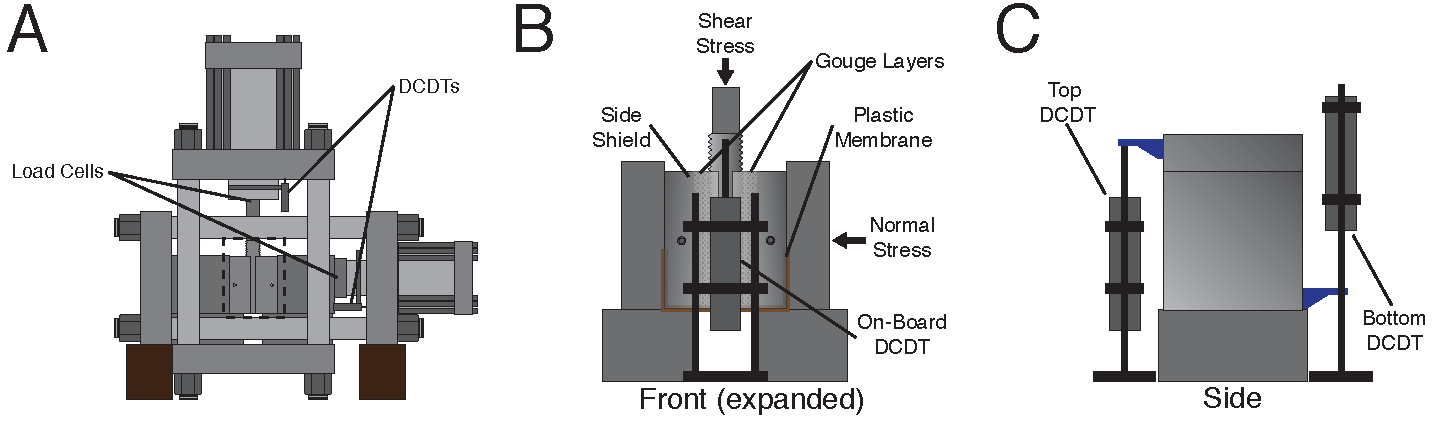
\includegraphics[scale=0.6]{chap_slow_slip_details/Figure_1.pdf}
   	\caption{A) The biaxial shearing apparatus with locations of load and displacement sensors indicated. The sample area is outlined with a dashed line. B) The double-direct-shear sample with an on-board displacement transducer mounted to the top of the center block and referenced to the base of the apparatus. C) A side view of the sample setup shows that an inverted displacement transducer is fitted on the back of the sample to measure the fault displacement at the bottom of the center block.}
  	\label{Figure_1}
\end{figure}
% End Figure %

\clearpage

% Figure %
\begin{figure}[H]
	\centering
		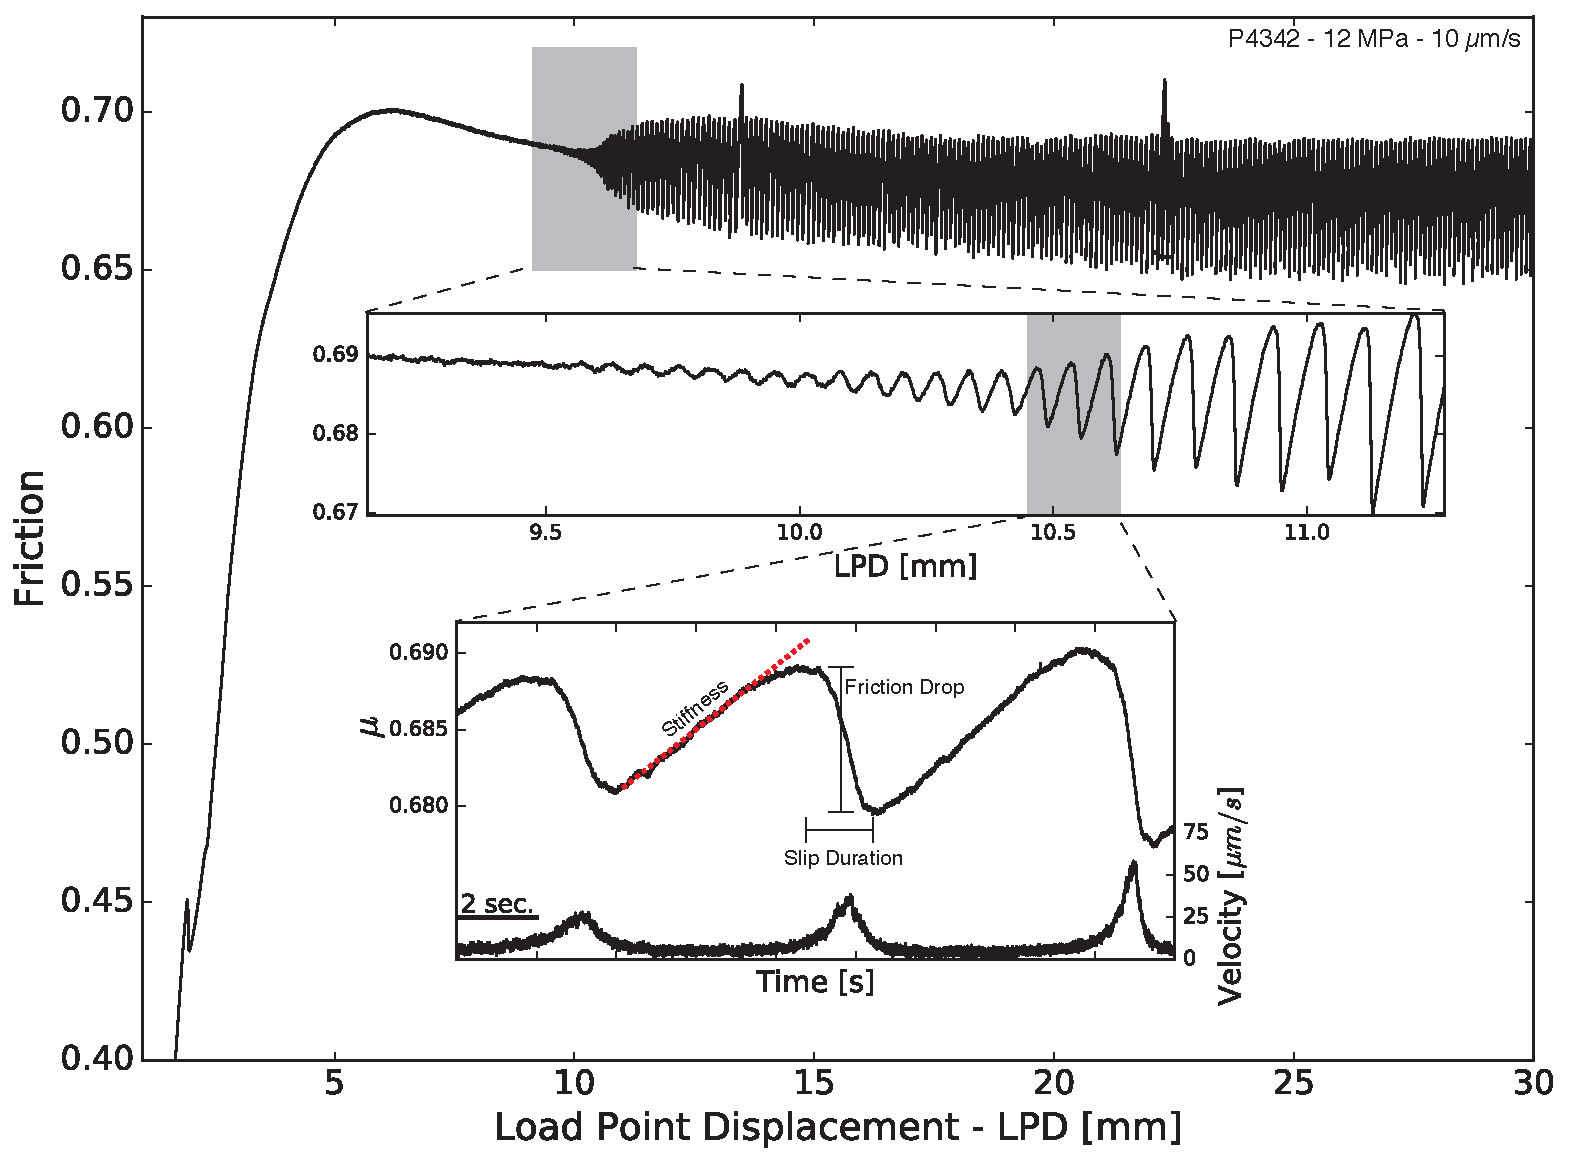
\includegraphics[scale=0.5]{chap_slow_slip_details/Figure_2.pdf}
   	\caption{Slow slip events spontaneously begin at approximately $10$ mm load point displacement. The onset of the events is emergent, evolving to their final steady-state over $20-30$ events. The friction drop of an event is defined as the difference between the maximum friction after the last event and the minimum friction prior to the next event. Slip duration is the time elapsed between these two friction values. The stiffness of a stick-slip event is the slope of the best-fit line to the loading portion of an event in a friction-displacement plot (shown here in time for convenience, only differing from the stiffness by a constant given a fixed load point velocity).}
  	\label{Figure_2}
\end{figure}
% End Figure %

\clearpage

% Figure %
\begin{figure}
	\centering
		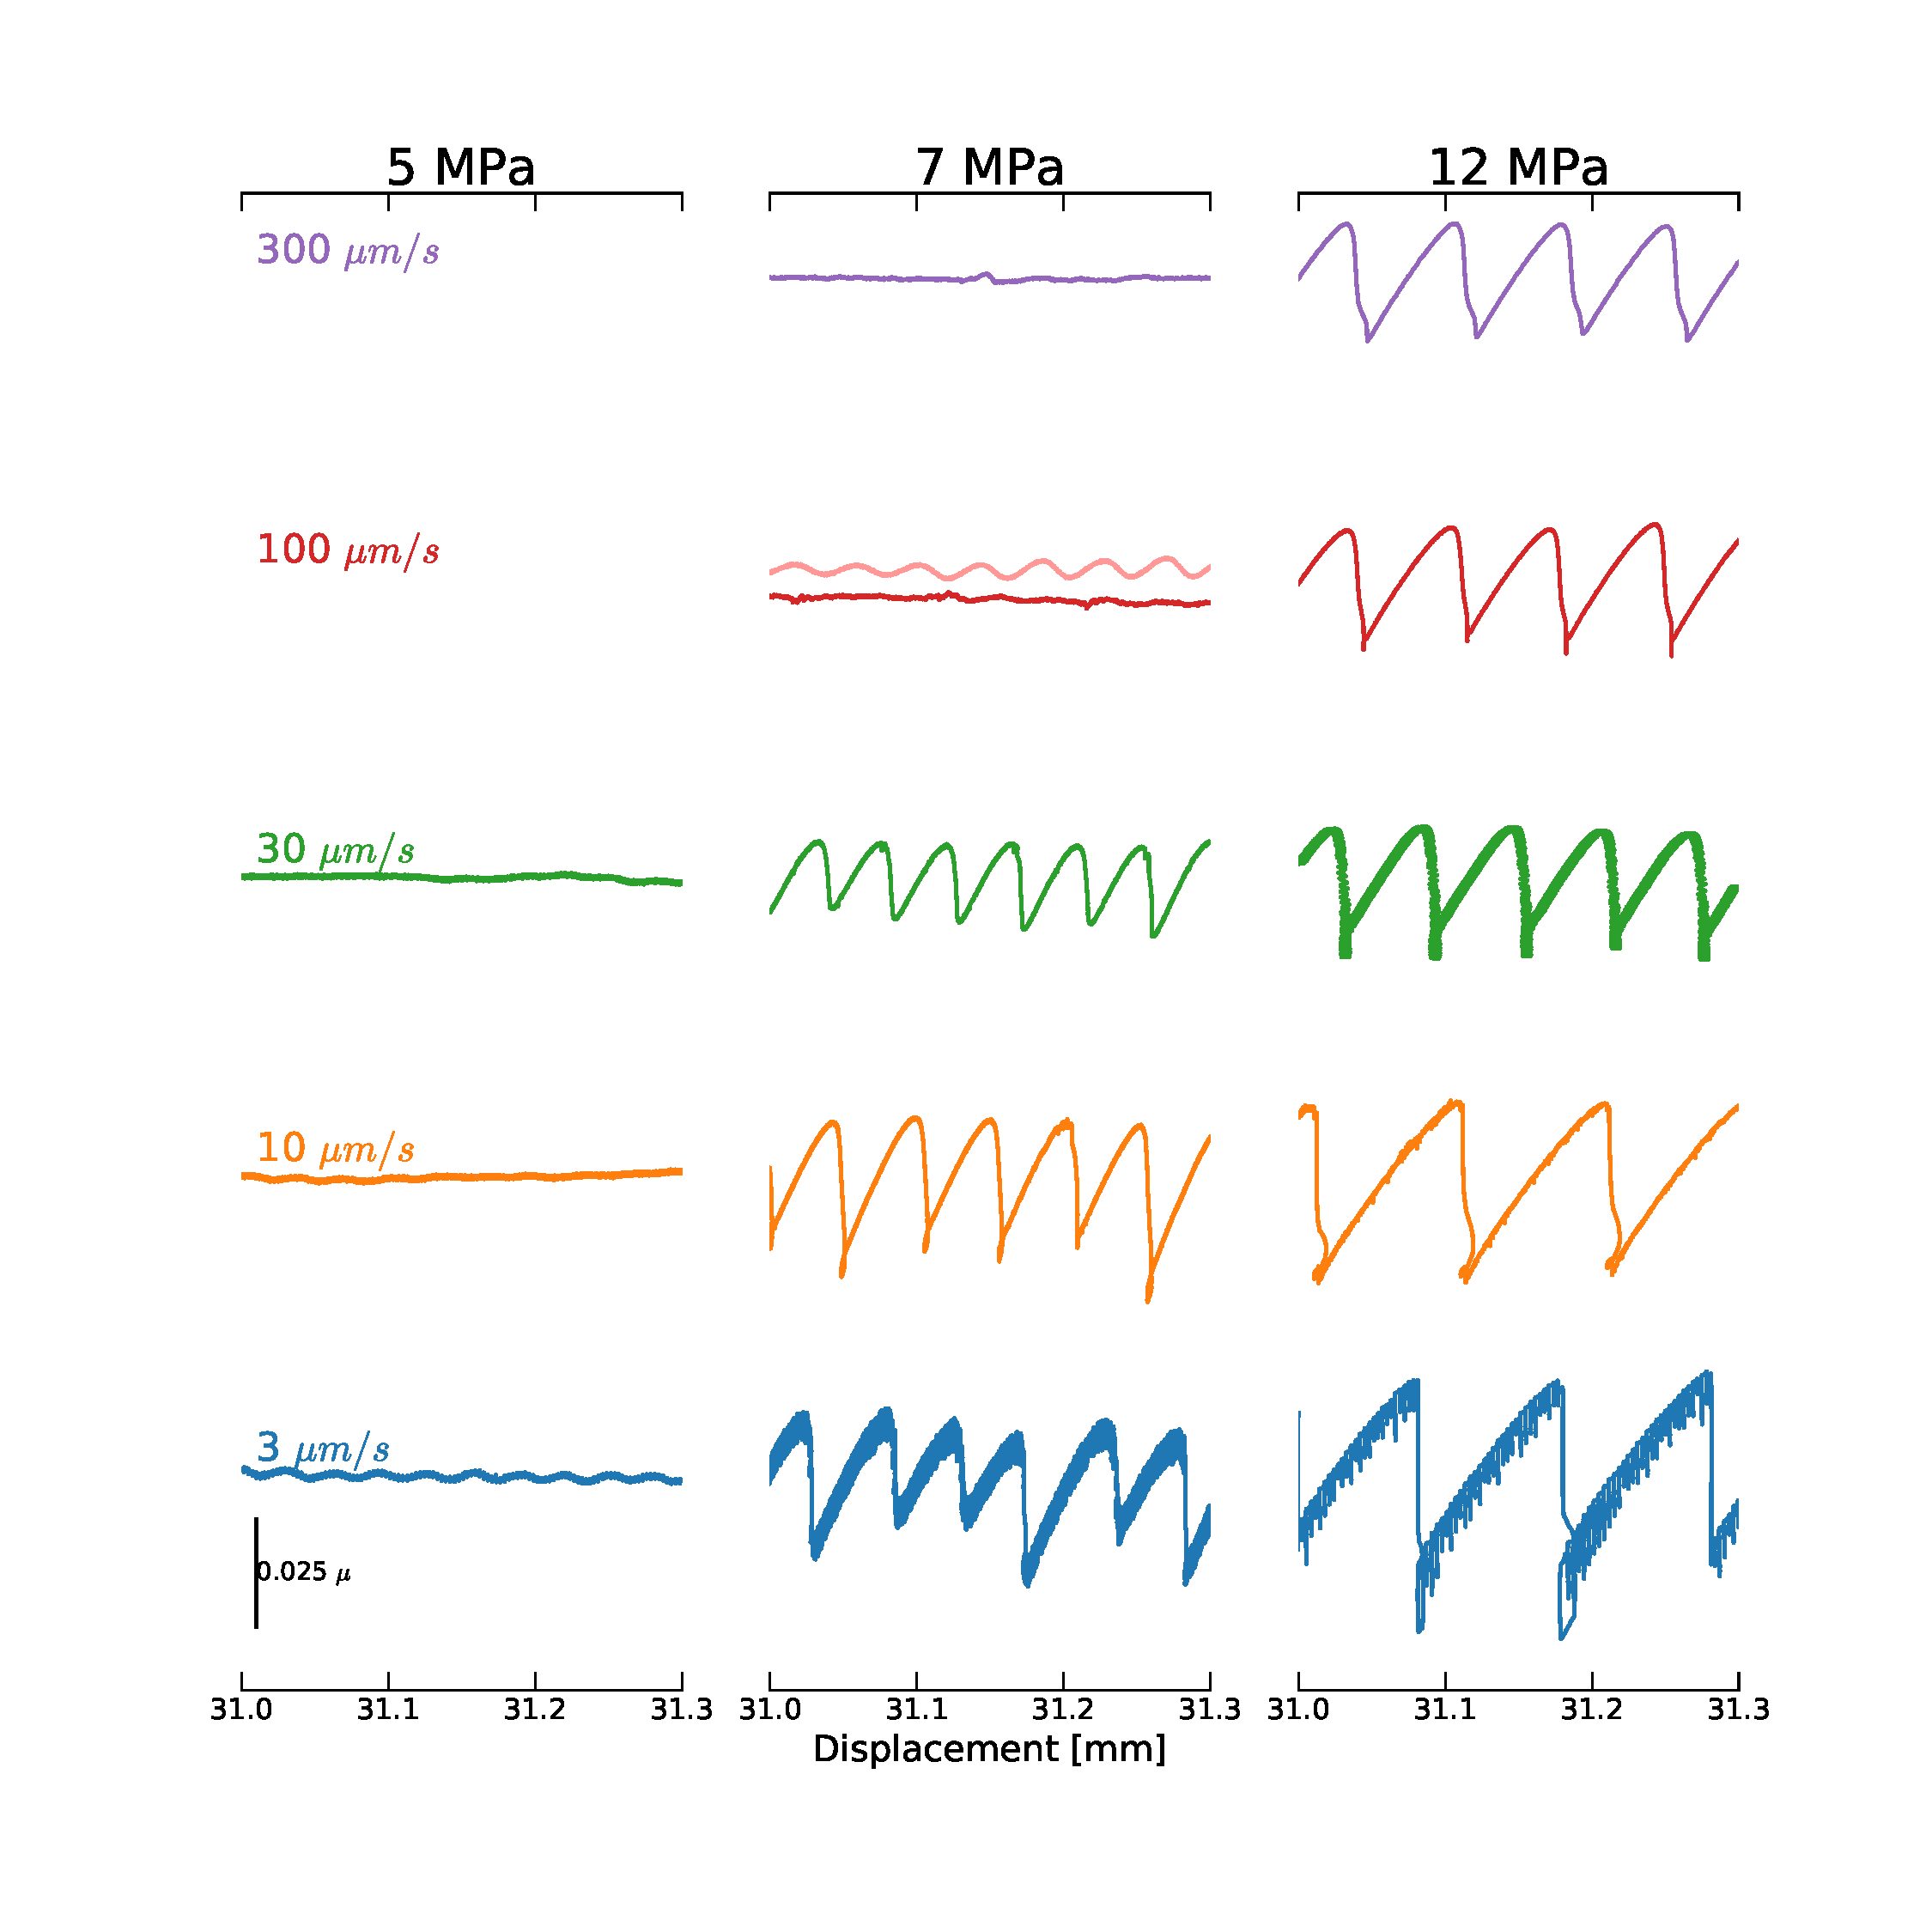
\includegraphics[scale=0.4]{chap_slow_slip_details/Figure_3.pdf}
   	\caption{Increased driving velocity or reduced normal stress can cause a system to become stable. Each experiment was run at a constant driving velocity and normal stress for its duration. Two experiments at $7$ MPa and $100 \mu\text{m/s}$ show different behaviors, indicating that those conditions are at the stability boundary.}
  	\label{Figure_3}
\end{figure}
% End Figure %

\clearpage

% Figure %
\begin{figure}[H]
	\centering
		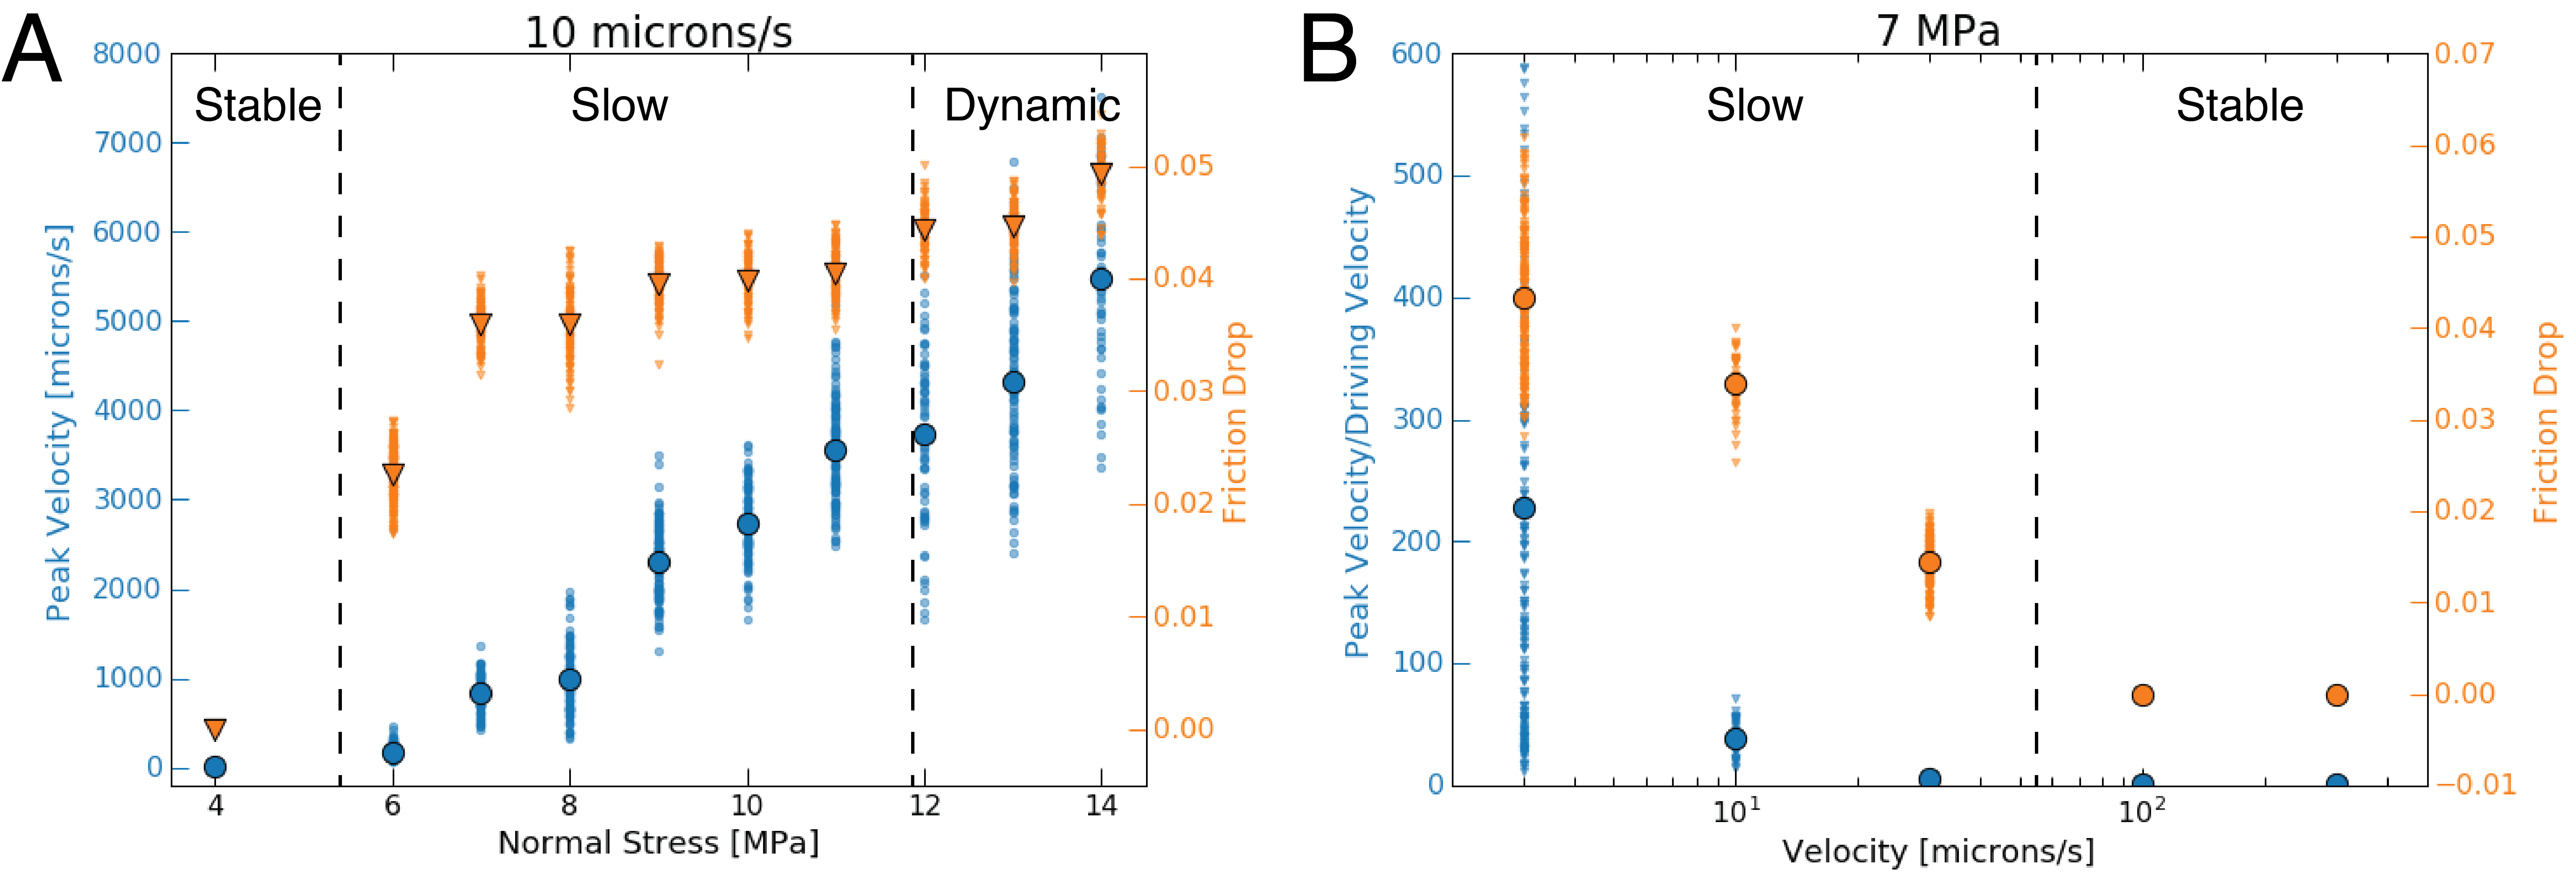
\includegraphics[scale=0.3]{chap_slow_slip_details/Figure_4.pdf}
   	\caption{A) At a fixed driving velocity of $10 \mu\text{m/s}$, increasing normal stress decreases the critical stiffness ratio and makes the system more unstable. Friction drop and peak slip velocity both increase with increasing normal stress. B) For a fixed normal stress, higher driving velocities result in lower friction drops and normalized peak friction drops as the system gets closer to being stable until it becomes stable near $100 \mu\text{m/s}$.}
  	\label{Figure_4}
\end{figure}
% End Figure %

\clearpage

% Figure %
\begin{figure}[H]
	\centering
		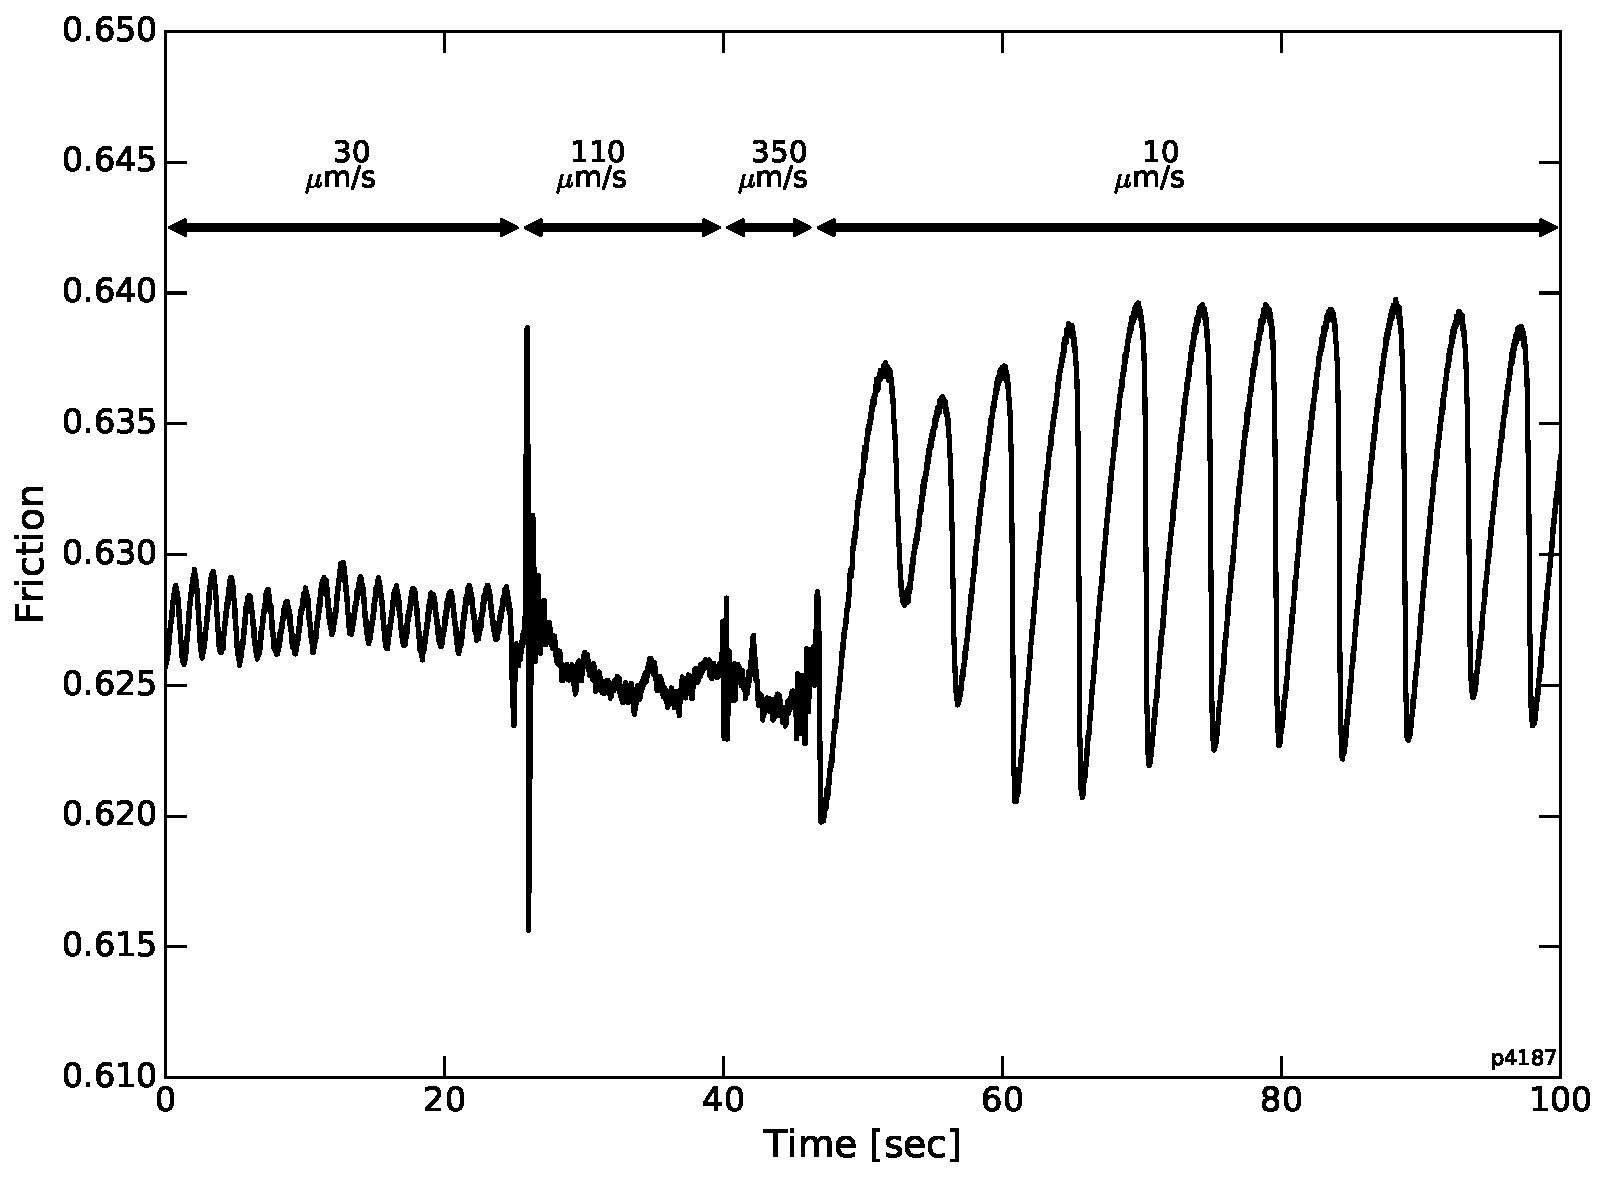
\includegraphics[scale=0.5]{chap_slow_slip_details/Figure_5.pdf}
   	\caption{In a given experiment, the stability of the system can be modified by changing the load-point velocity. As the load point velocity is increased from $30 \mu\text{m/s}$ to $100 \mu\text{m/s}$ and $350 \mu\text{m/s}$ the system transitions from small slow slipping stress oscillations to stable sliding. Upon an abrupt reduction in velocity to $10 \mu\text{m/s}$, the fault switches back to slow-slip behavior, but this time with a larger amplitude due to the lower driving velocity.}
  	\label{Figure_5}
\end{figure}
% End Figure %

\clearpage

% Figure %
\begin{figure}[H]
	\centering
		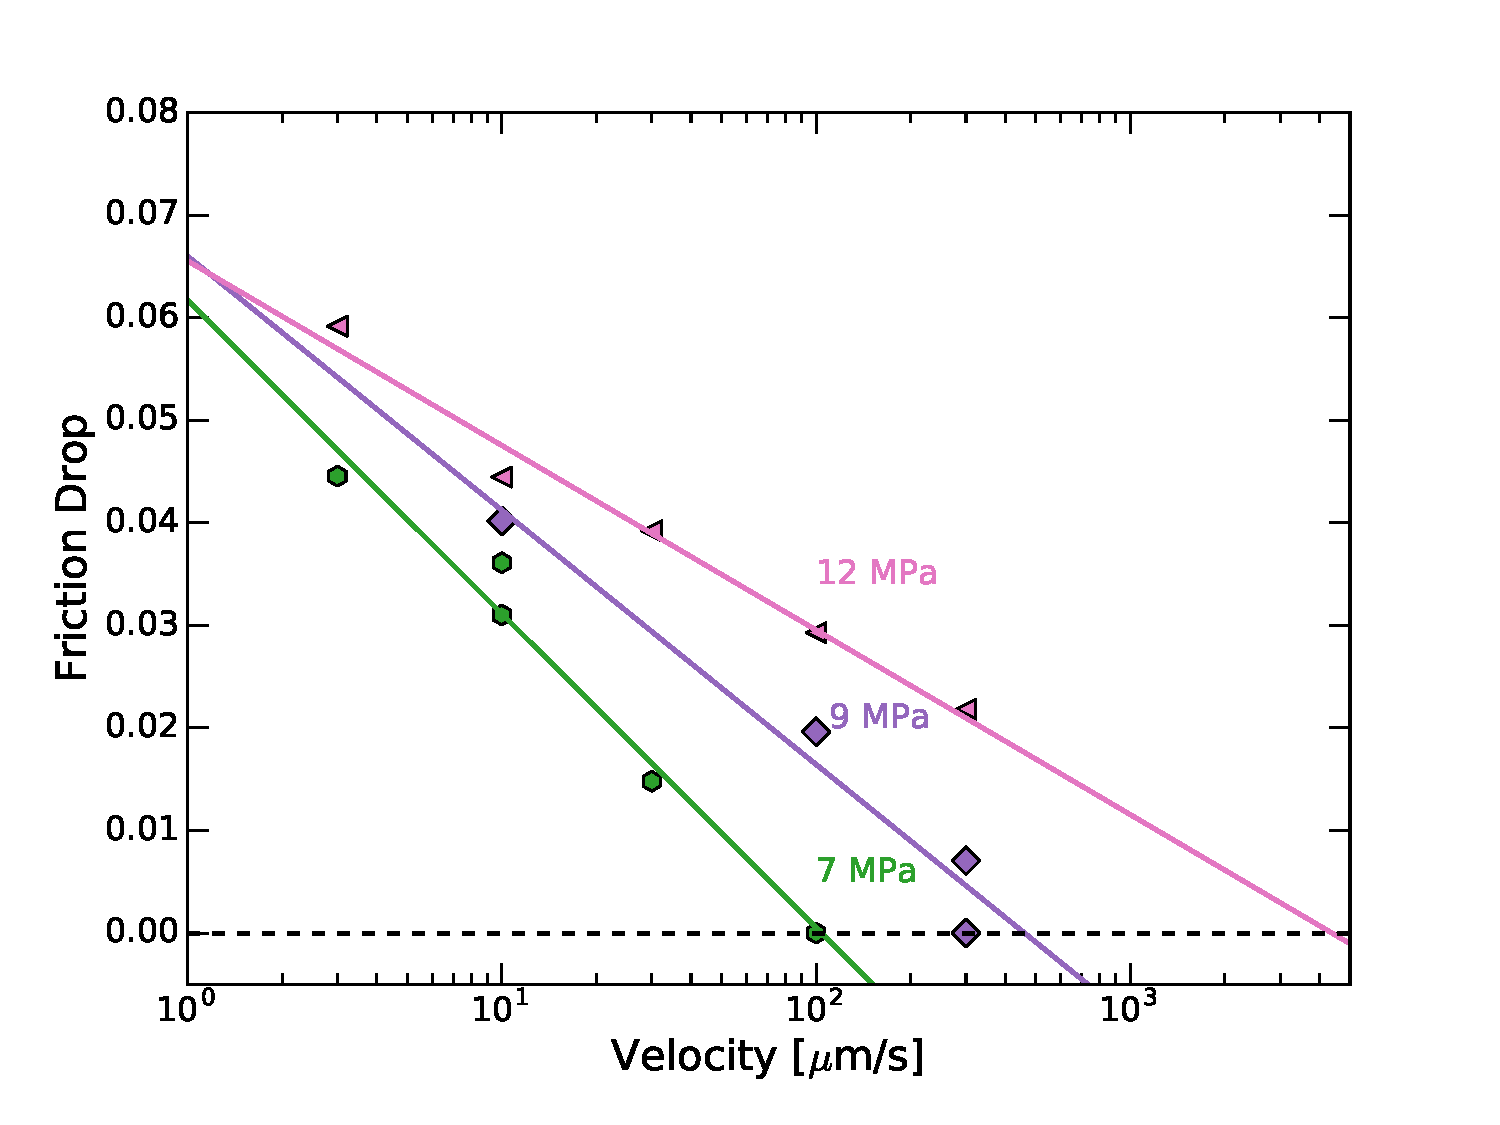
\includegraphics[scale=0.55]{chap_slow_slip_details/Figure_6.pdf}
   	\caption{Friction drop scales logarithmically with load point velocity. As the normal stress increases and the critical stiffness ratio decreases, the systems become more unstable and has higher friction drops at a given velocity. The scaling constant appears to decrease with higher normal stress, suggesting that higher normal stresses the friction drop is more weakly dependent on velocity.}
  	\label{Figure_6}
\end{figure}
% End Figure %

\clearpage

% Figure %
\begin{figure}[H]
	\centering
		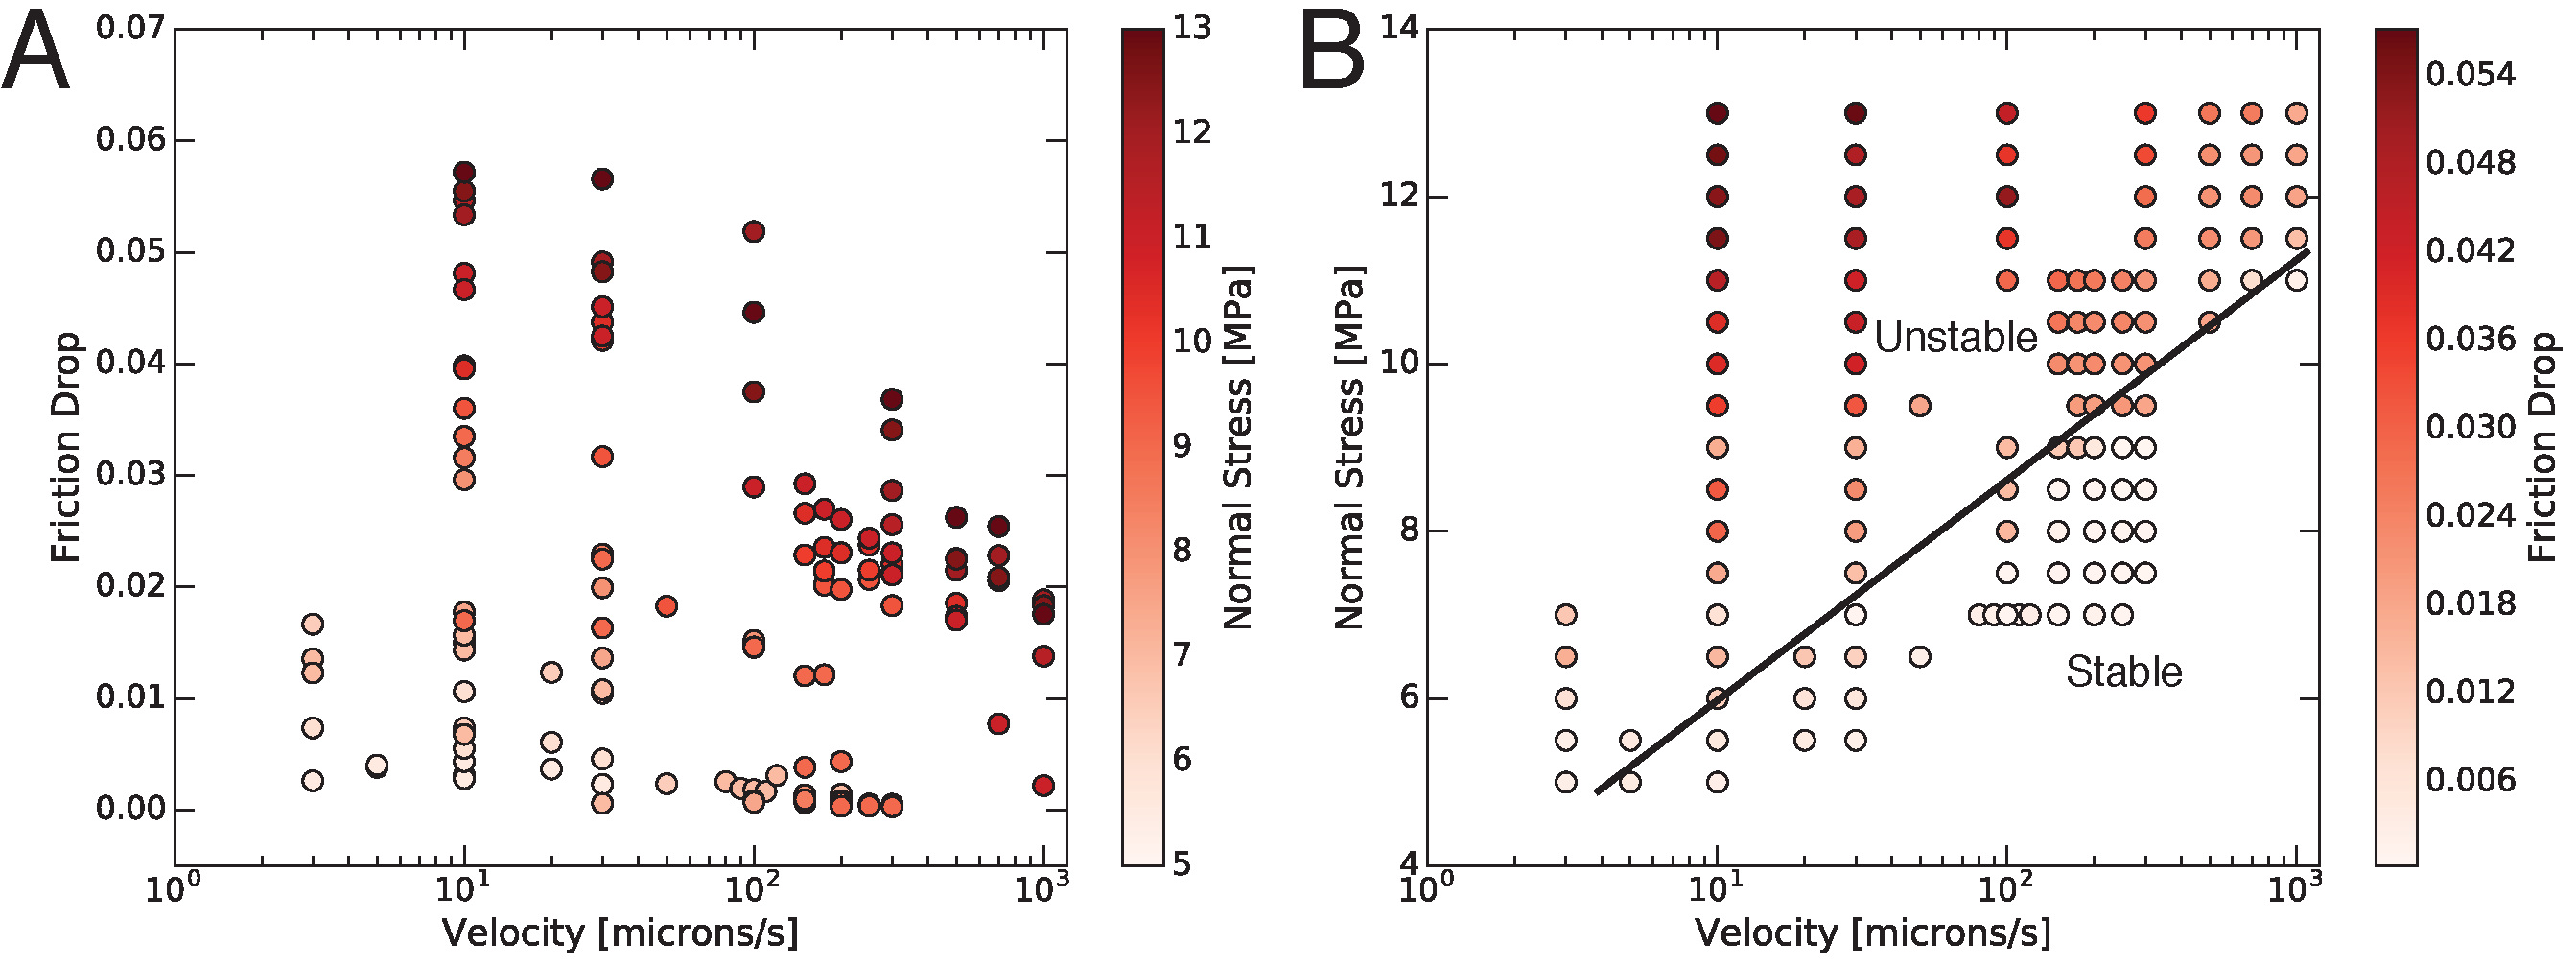
\includegraphics[scale=0.3]{chap_slow_slip_details/Figure_7.pdf}
   	\caption{A) Friction drops decrease with increased loading velocity in a log-linear fashion. B) The division between stable (near zero friction drop) and unstable (significant friction drop) conditions is apparent as a nearly straight boundary in the normal stress - driving velocity space. For a given normal stress, the transition can be seen in the whitening of the data points.}
  	\label{Figure_7}
\end{figure}
% End Figure %

\clearpage

% Figure %
\begin{figure}[H]
	\centering
		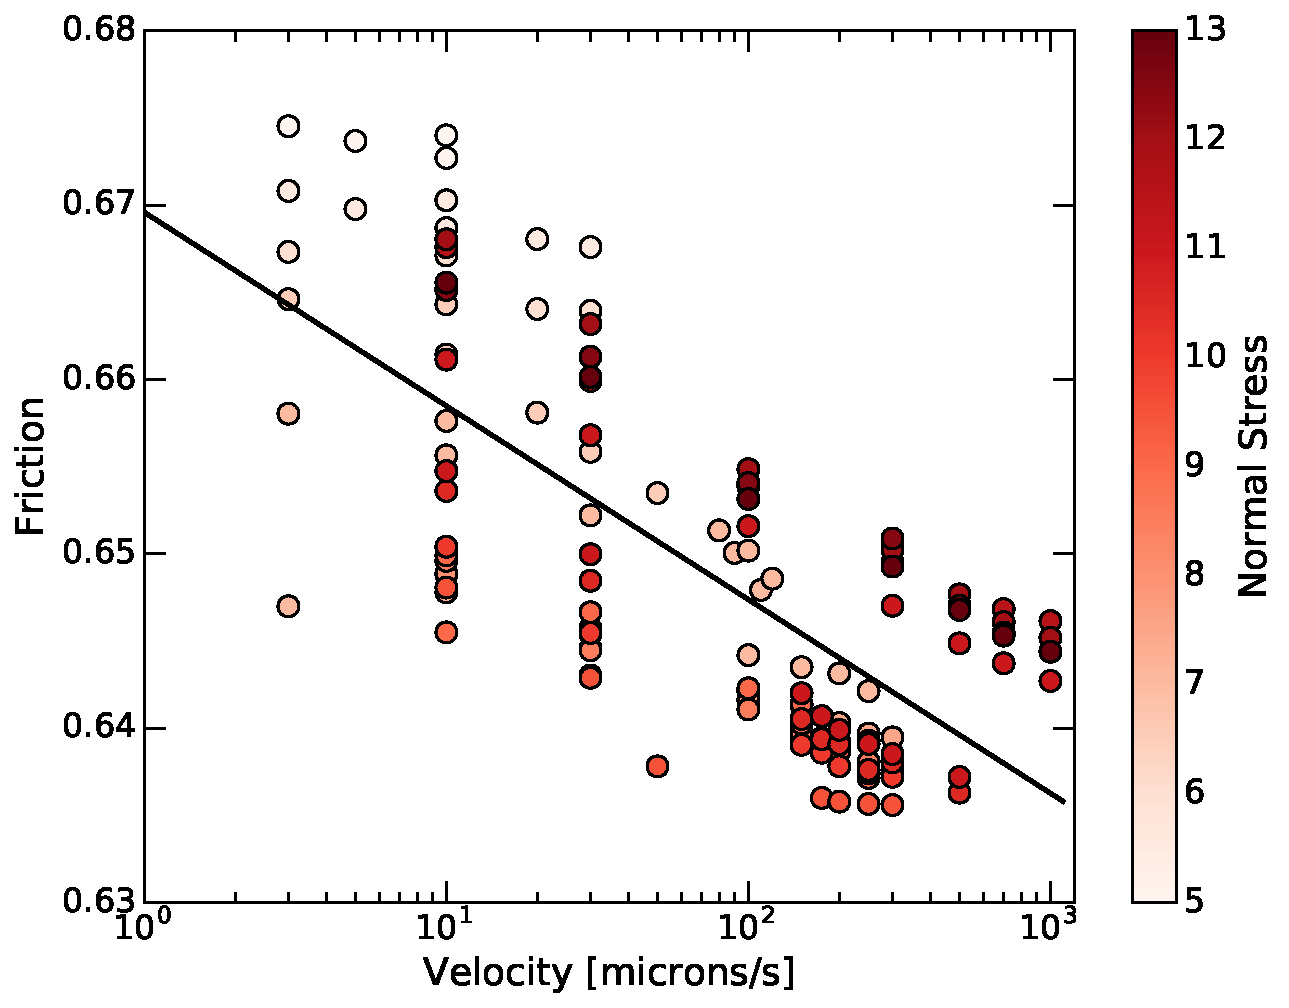
\includegraphics[scale=0.6]{chap_slow_slip_details/Figure_8.pdf}
   	\caption{Mean friction at a range of velocities for experiments with normal stresses ranging from $5-13$ MPa show a linear decrease in friction with increasing velocity. The slope of this line is $(a-b)$ and has a value of $-0.00482$ for all data shown.}
  	\label{Figure_8}
\end{figure}
% End Figure %

\clearpage

% Figure %
\begin{figure}[H]
	\centering
		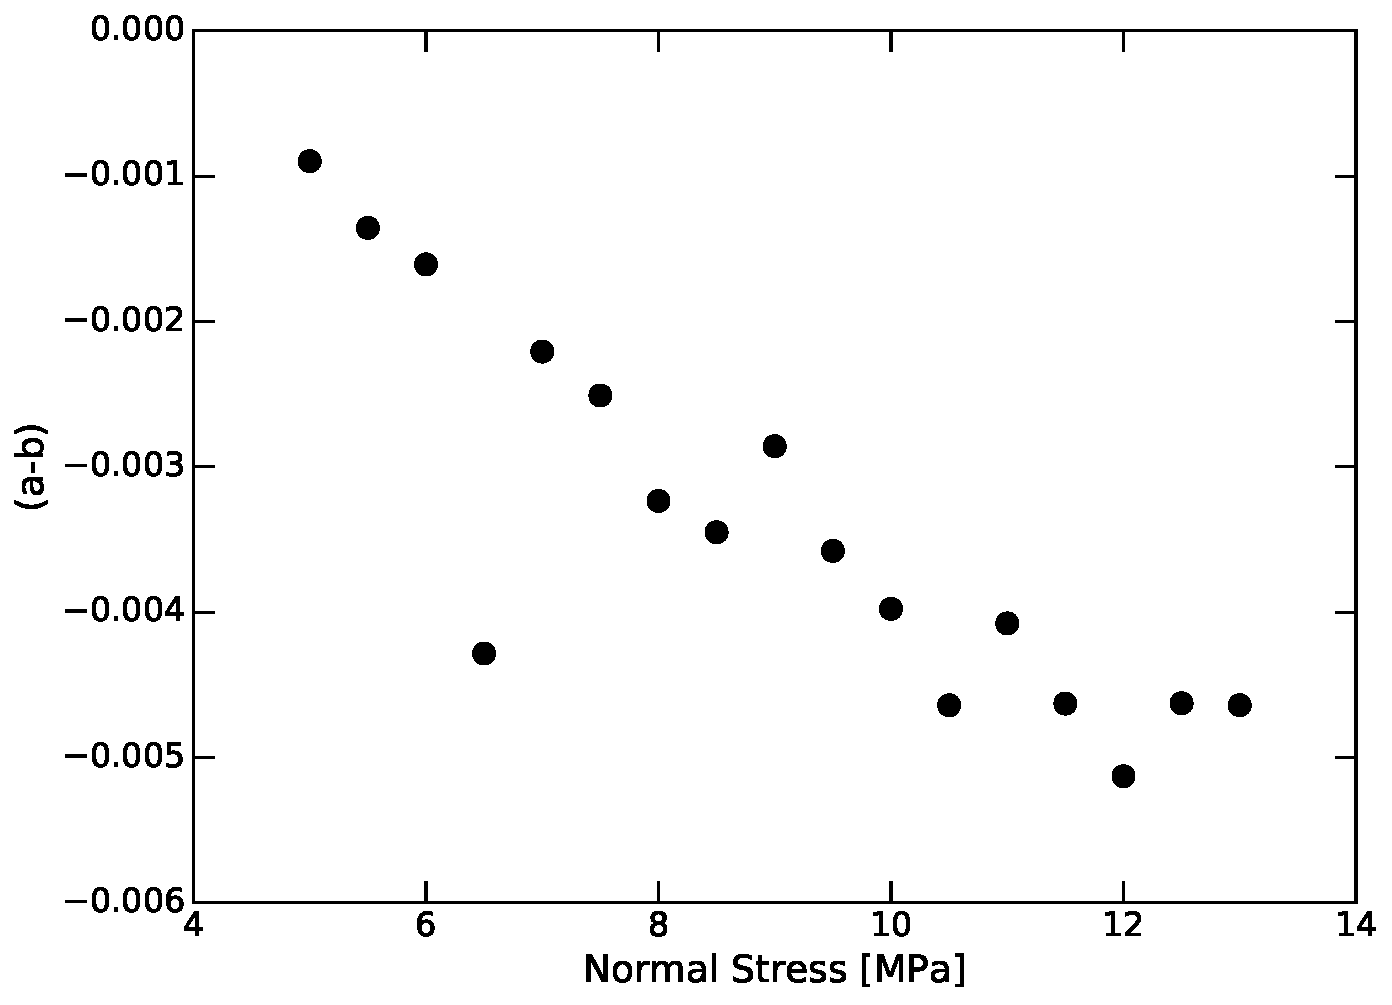
\includegraphics[scale=0.6]{chap_slow_slip_details/Figure_9.pdf}
   	\caption{By fitting the mean friction at multiple velocities at each normal stress, $(a-b)$ estimates show a linear decrease in $(a-b)$ with normal stress. Assuming that all other factors remain constant, this would mean at a given velocity, an increase in normal stress would reduce $(a-b)$ making the system more unstable. This effect would be superimposed on increase of $k_c$ with normal stress.}
  	\label{Figure_9}
\end{figure}
% End Figure %

\clearpage

% Figure %
\begin{figure}[H]
	\centering
		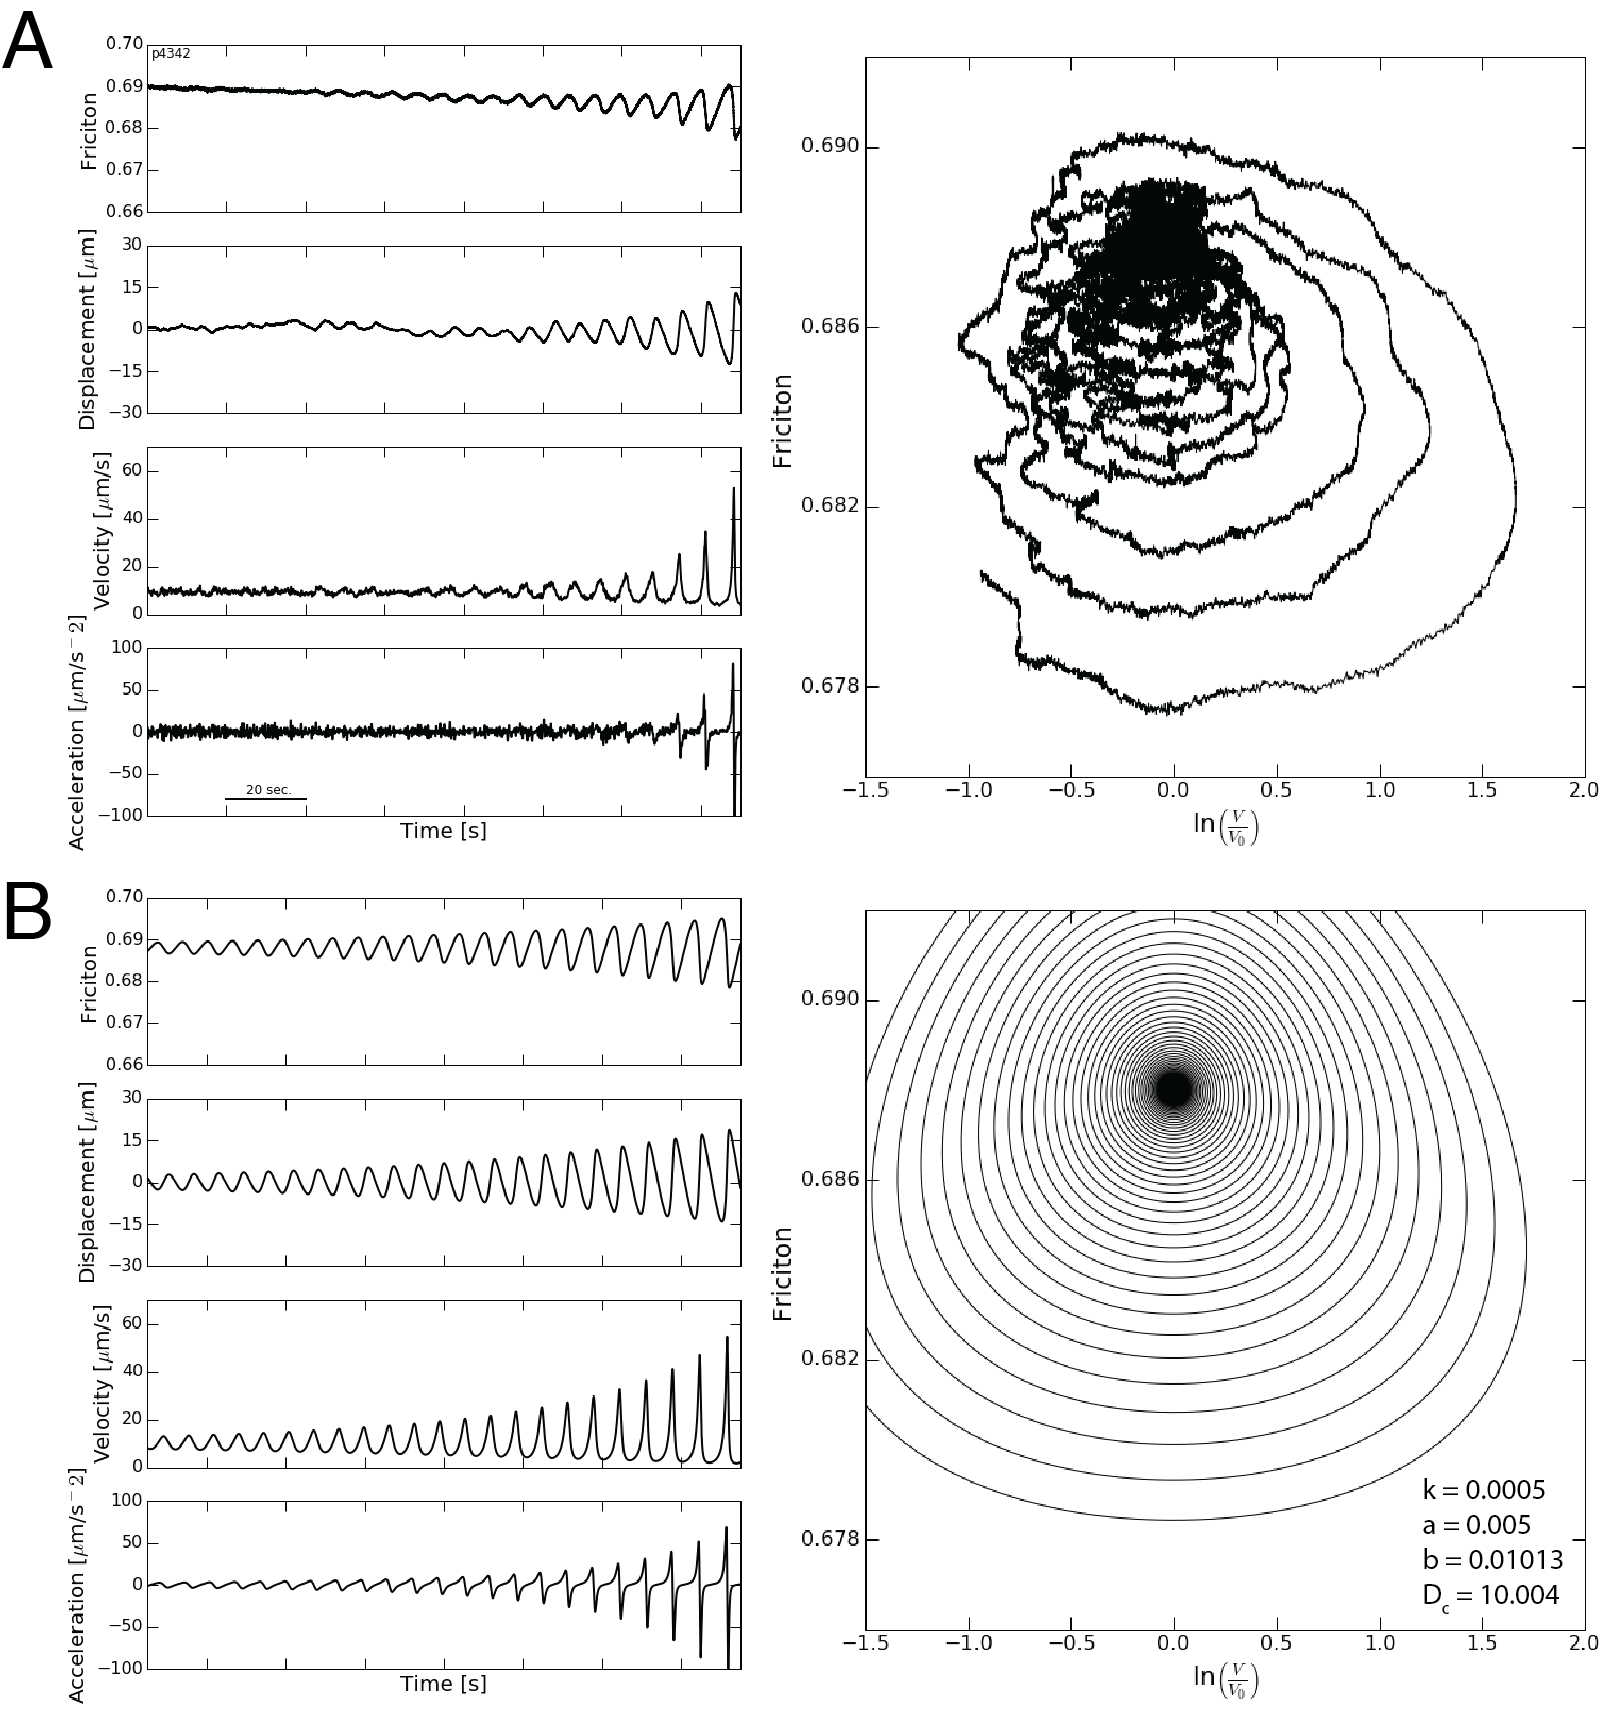
\includegraphics[scale=1.0]{chap_slow_slip_details/Figure_10.png}
   	\caption{The onset of instability occurs over tens of slip cycles in our data (A) and a simple rate-and-state friction model (B). Each successive friction drop is larger with increased slip displacement, velocity, and acceleration. The acceleration/deceleration magnitudes are nearly identical for these nearly sinusoidal onset events. In the model, the behavior was very sensitive to small perturbations in $(a-b)$ and $D_c$.}
  	\label{Figure_10}
\end{figure}
% End Figure %

\clearpage

% Figure %
\begin{figure}[H]
	\centering
		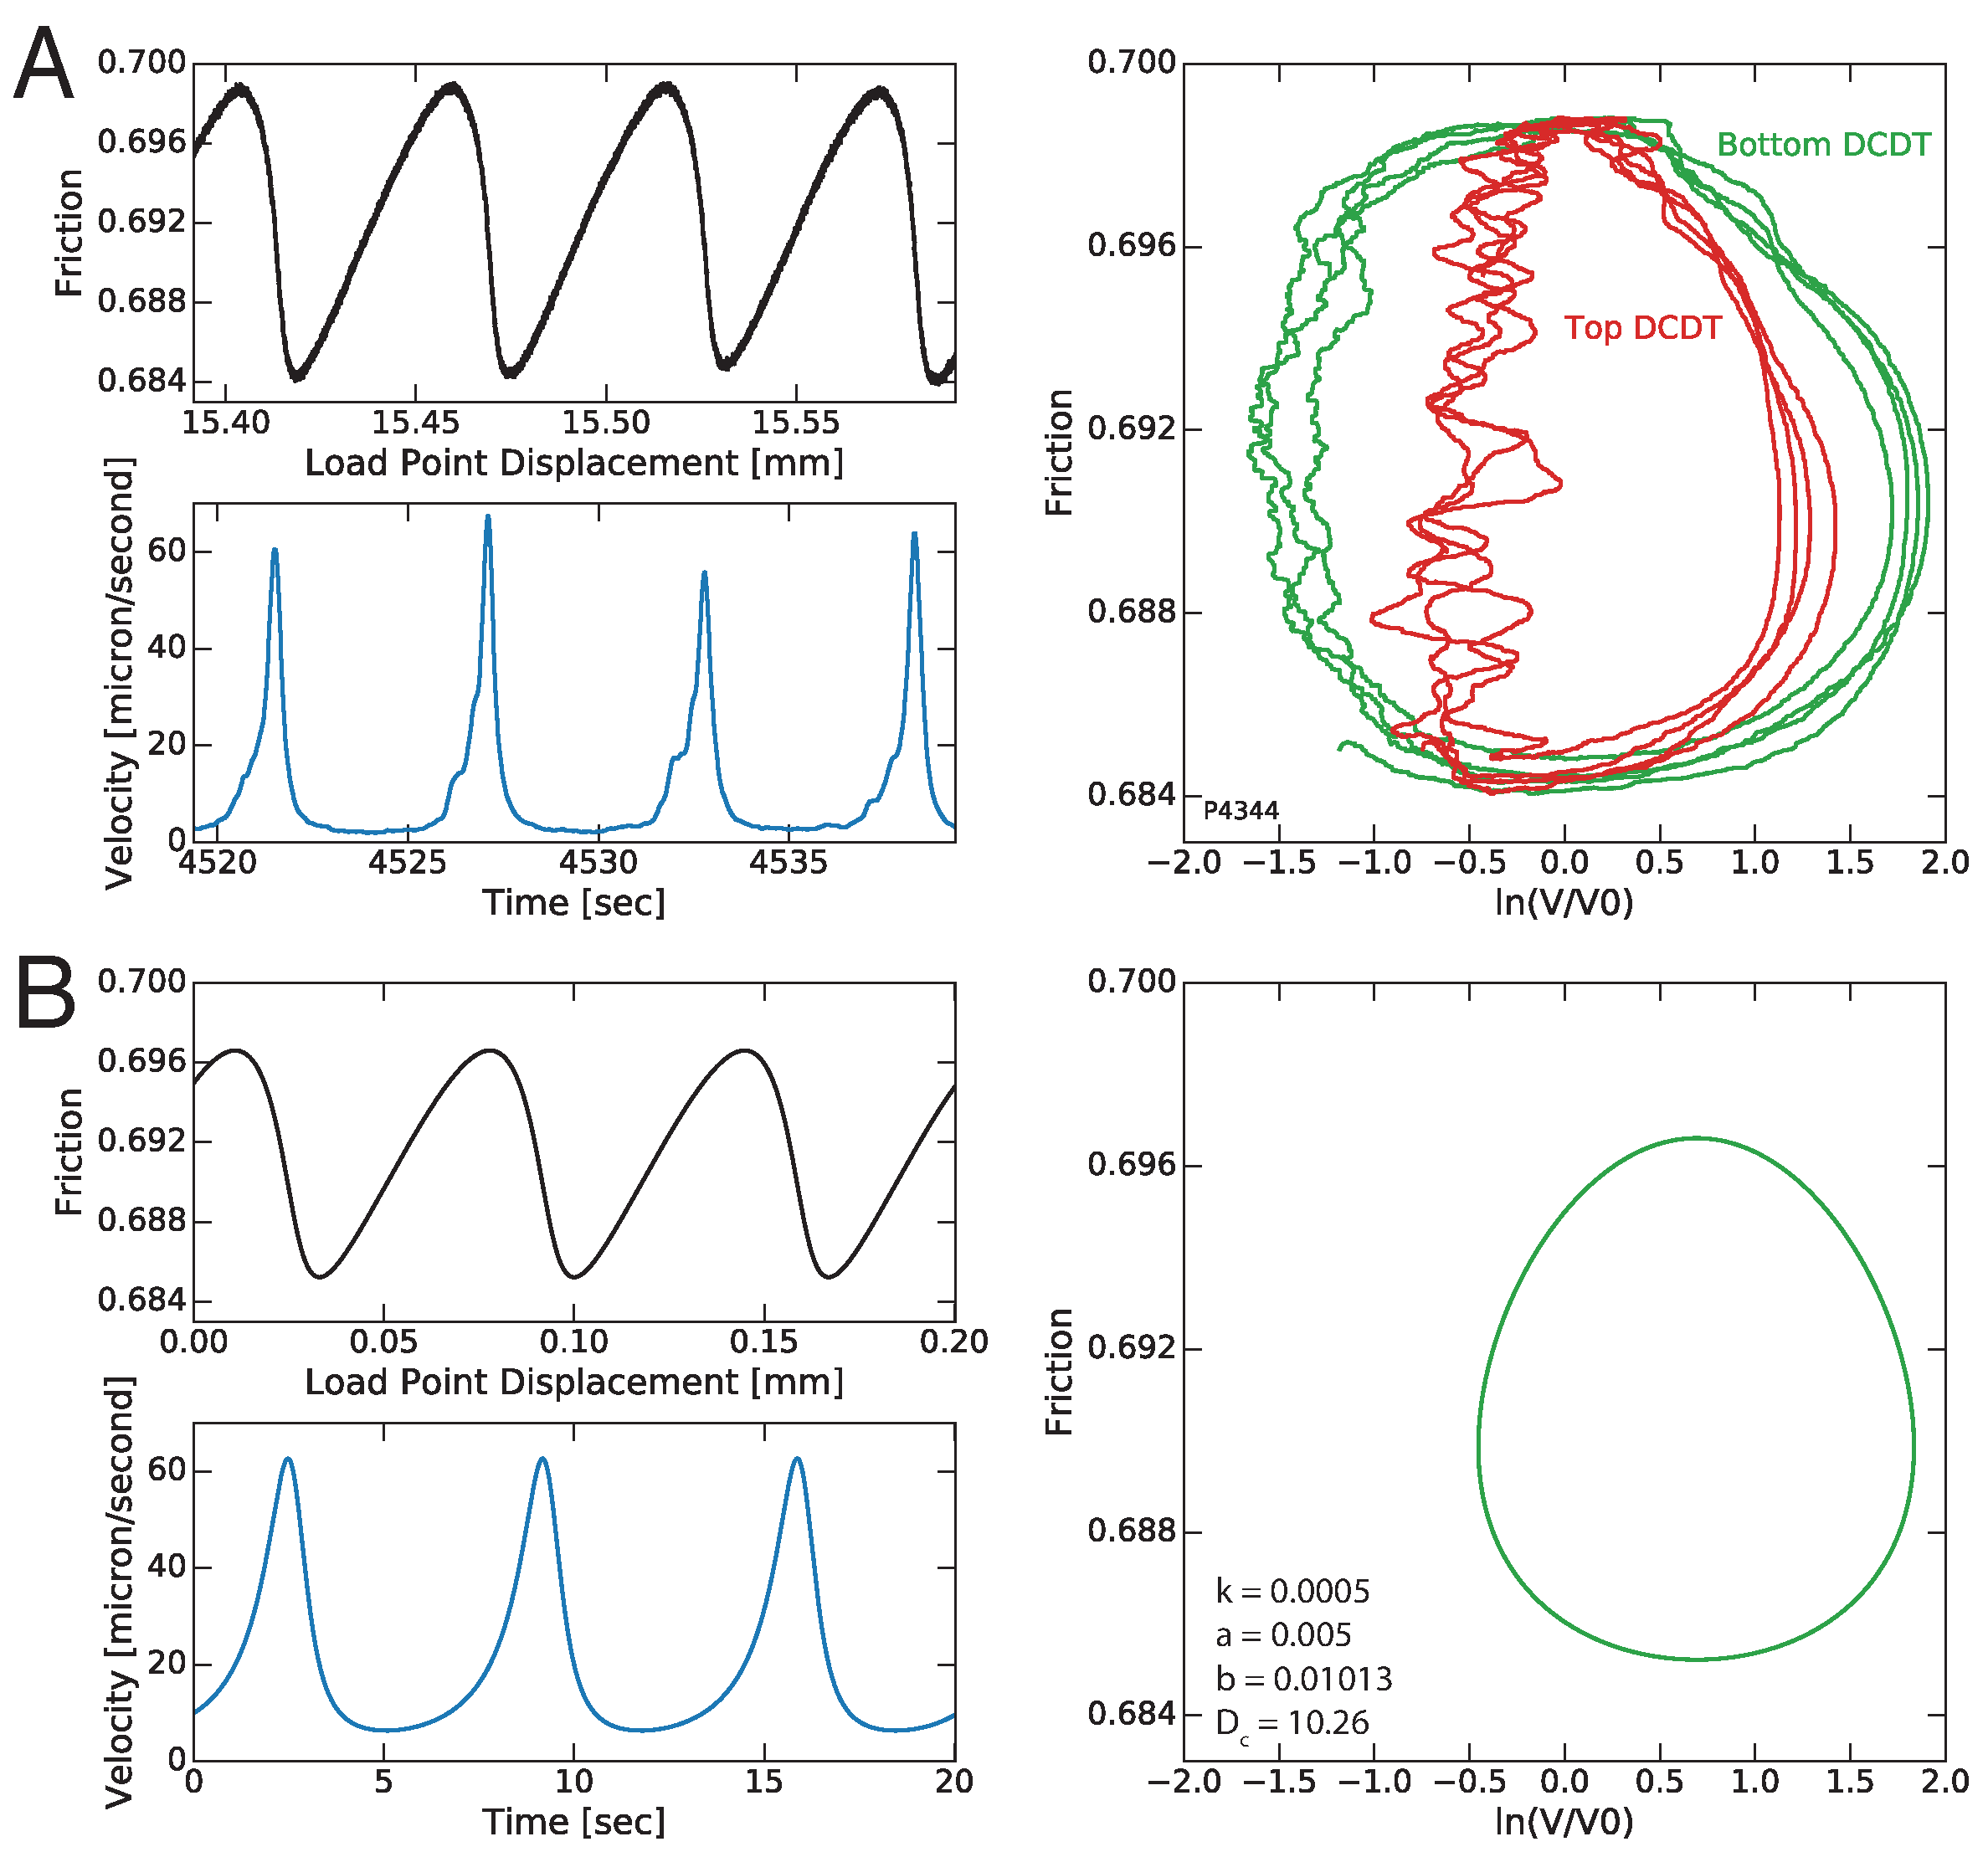
\includegraphics[scale=0.35]{chap_slow_slip_details/Figure_11.pdf}
   	\caption{A) An experimental plot of four slow-slip events, their time-friction curve, time-slider velocity curve, and phase plots. Notice that the top DCDT remains very close to the loading velocity, while the bottom DCDT becomes virtually stationary during the loading phase of the slip events. This indicates significant storage of strain energy in the forcing block. The bottom DCDT shows the slipping part of the experimental fault to slip faster than the top of the loading block, but with a nearly identical velocity profile. B) When setting $\kappa  = 1$ in a single state-variable rate-and-state friction model, a small perturbation will setup a limit cycle in which the system continually slow-slips, retracing the same path in phase space. The magnitude of the friction drop and peak slip velocity are dependent upon the size of velocity perturbation imposed on the system.}
  	\label{Figure_11}
\end{figure}
% End Figure %

\clearpage

% Figure %
\begin{figure}[H]
	\centering
		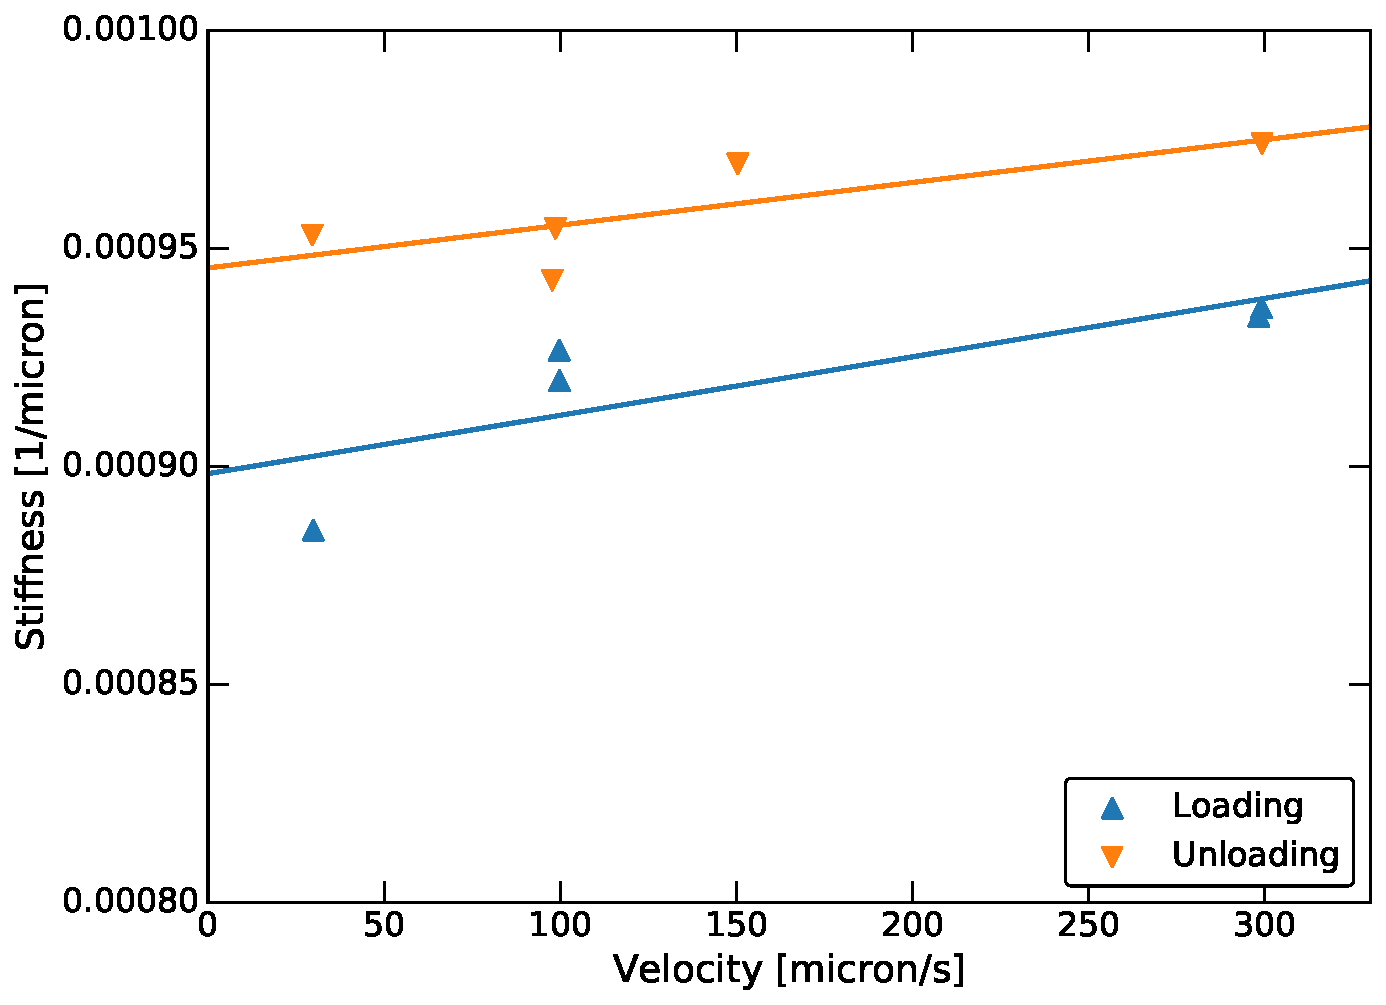
\includegraphics[scale=0.6]{chap_slow_slip_details/Figure_12.pdf}
   	\caption{The observed loading stiffness of our experimental system exhibits a slight increase with loading velocity.}
  	\label{Figure_12}
\end{figure}
% End Figure %

\clearpage

% Figure %
\begin{figure}[H]
	\centering
		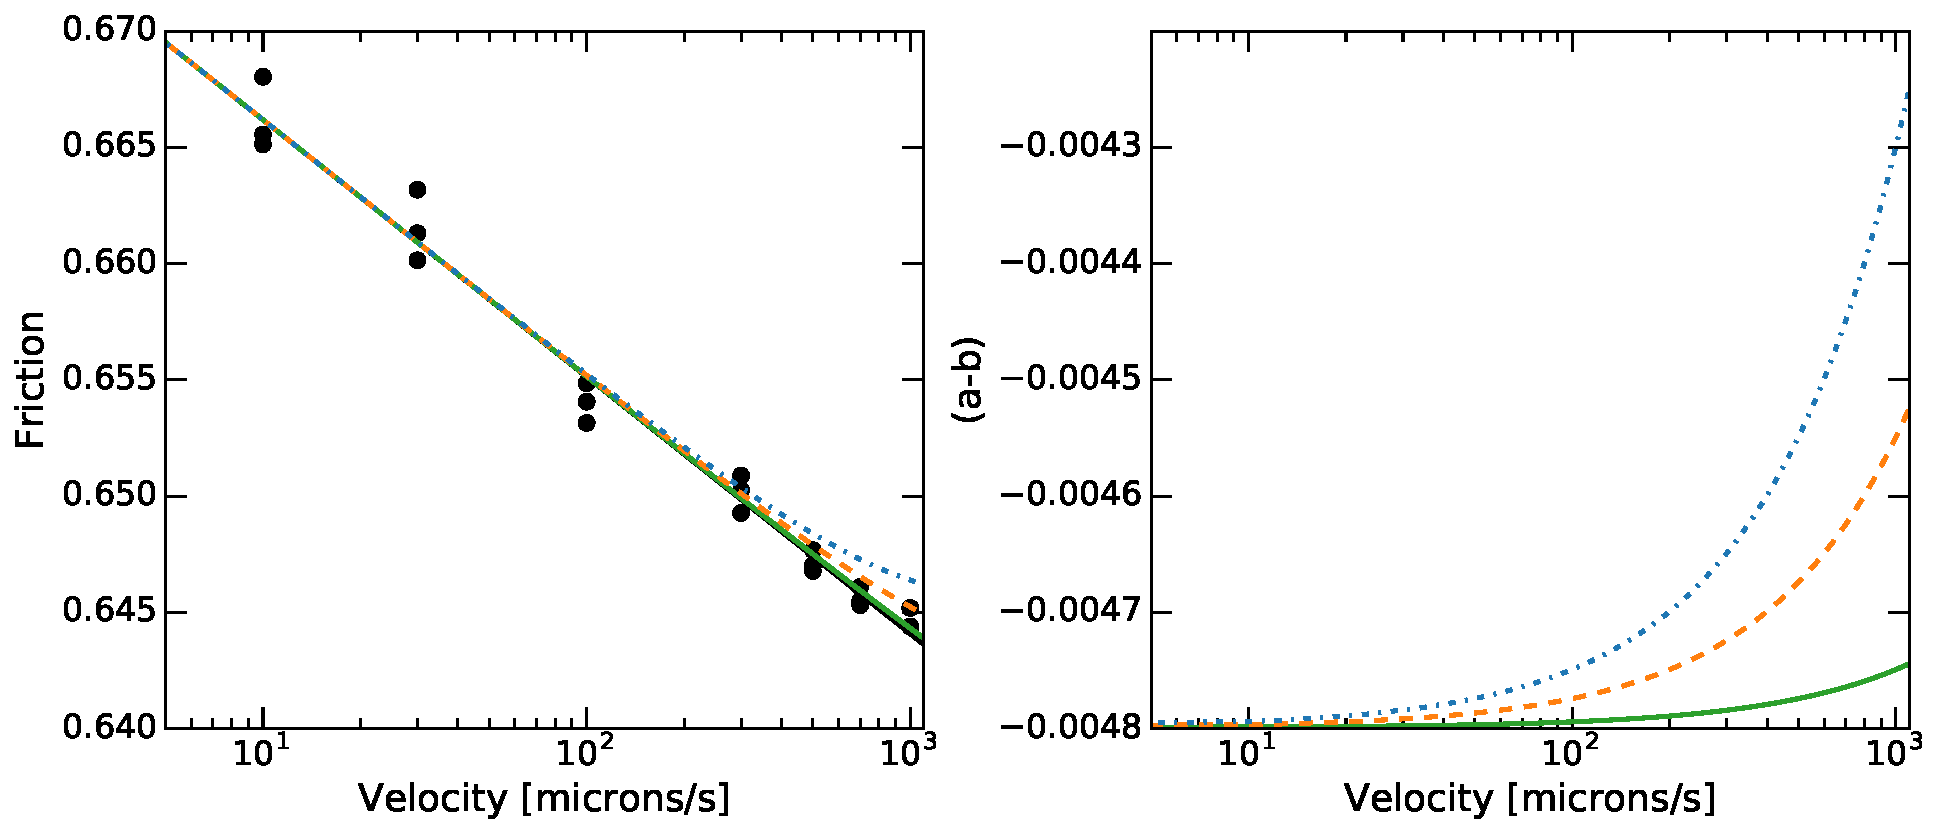
\includegraphics[scale=0.45]{chap_slow_slip_details/Figure_13.pdf}
   	\caption{Compiling data from $12-13$ MPa normal stress where $(a-b)$ is roughly constant, we see that small variations in $(a-b)$ are not ruled out by our data. Variations as small as $0.0005$ can make a significant difference in behavior when a system is near the stability boundary.}
  	\label{Figure_13}
\end{figure}
% End Figure %

\clearpage

% Figure %
\begin{figure}[H]
	\centering
		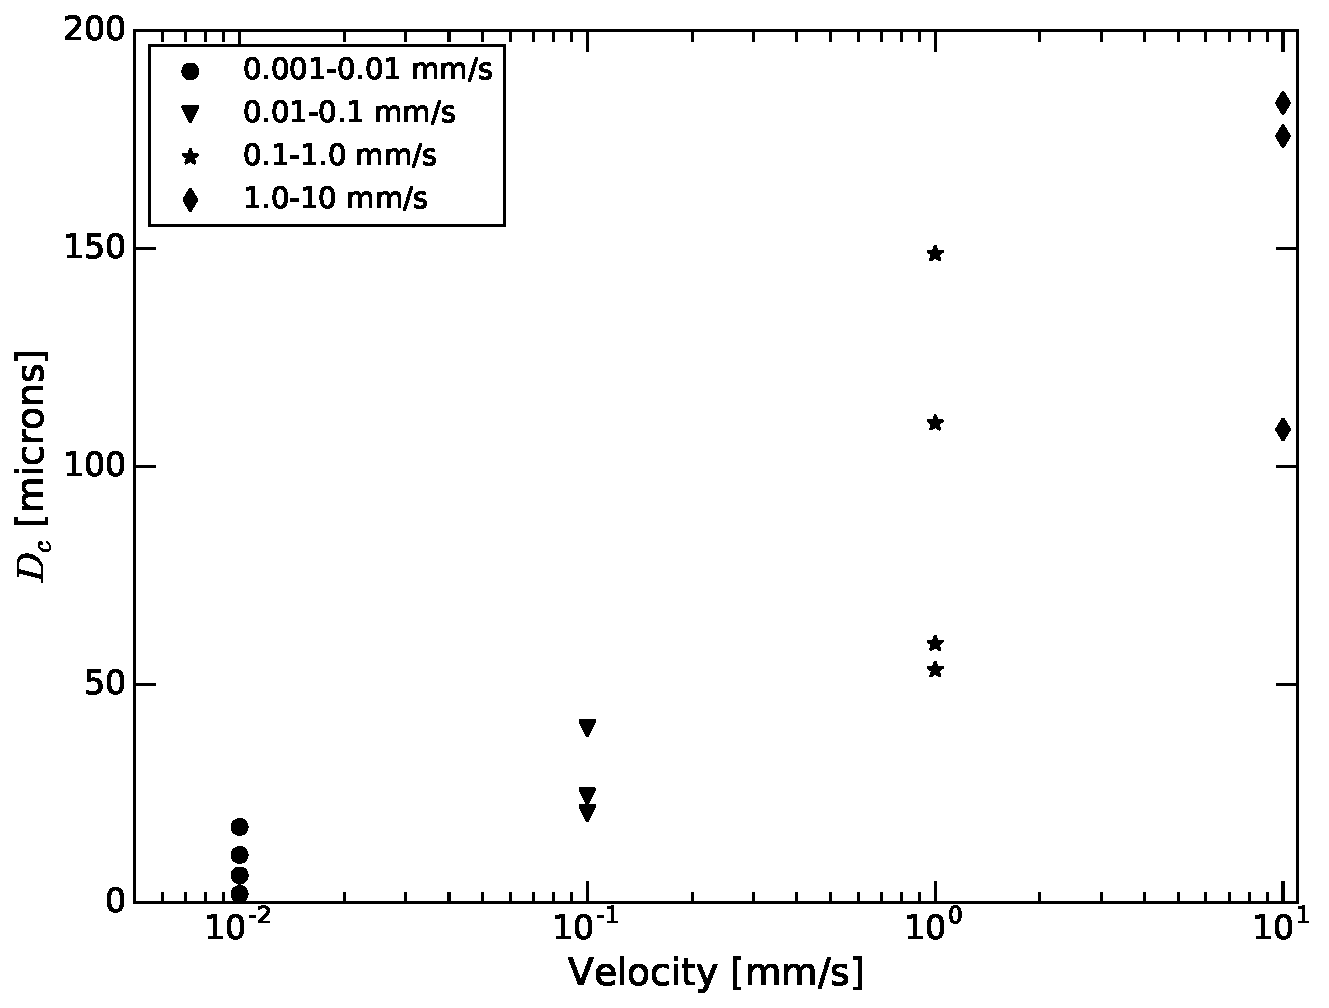
\includegraphics[scale=0.6]{chap_slow_slip_details/Figure_14.pdf}
   	\caption{The critical slip distance $D_c$, increases systemically with velocity in F110 experiments. While F110 is significantly larger than Min-U-Sil, it is of similar composition. Data from \cite{}Mair [1999]}
  	\label{Figure_14}
\end{figure}
% End Figure %

\clearpage

% Figure %
\begin{figure}[H]
	\centering
		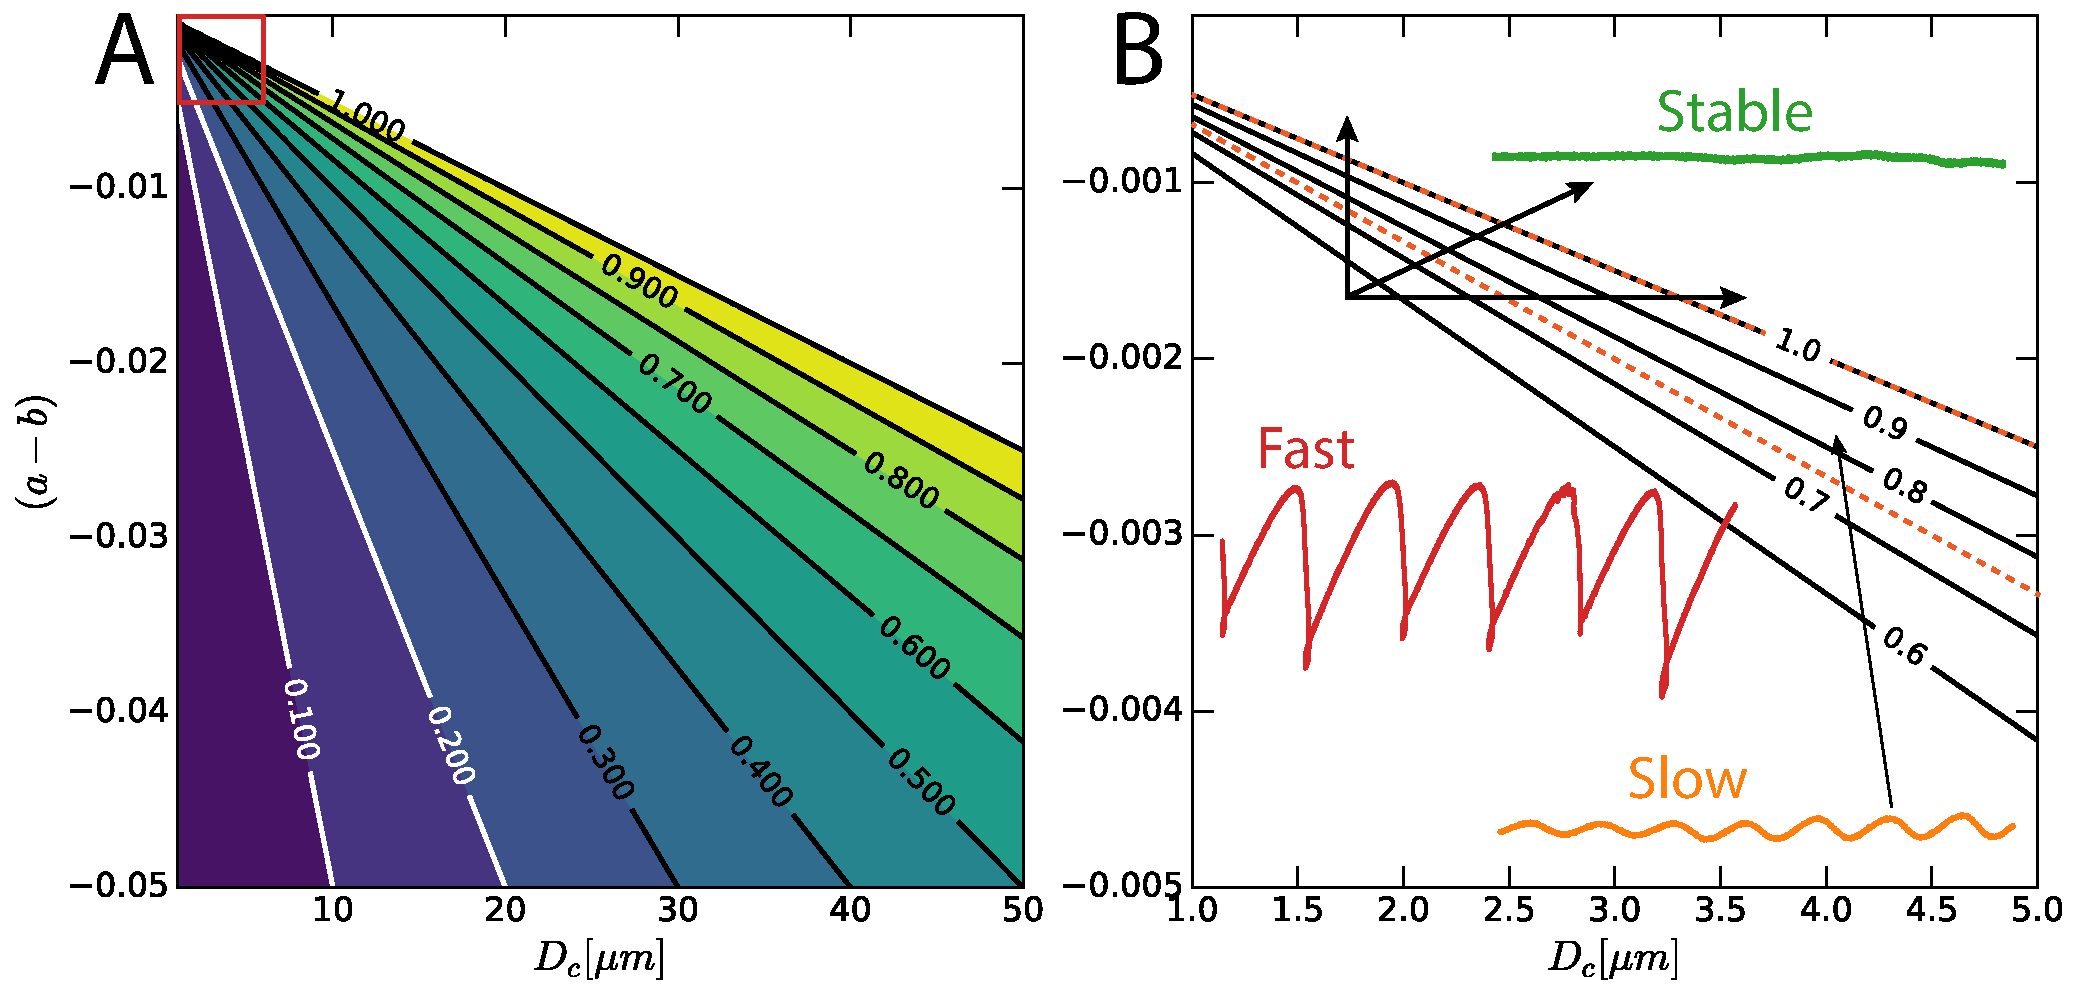
\includegraphics[scale=0.45]{chap_slow_slip_details/Figure_15.pdf}
   	\caption{The critical slip distance and frictional parameter $(a-b)$ trade off linearly to modify the critical stiffness ratio. When near the stability boundary, small changes in $(a-b)$ can produce stable behavior (vertical line), but changes of a few microns in $D_c$ can produce the same transition. The most likely scenario is that both parameters change with velocity, both increasing the stability of the system with increased driving velocity.}
  	\label{Figure_15}
\end{figure}
% End Figure %

\clearpage

% Figure %
\begin{figure}[H]
	\centering
		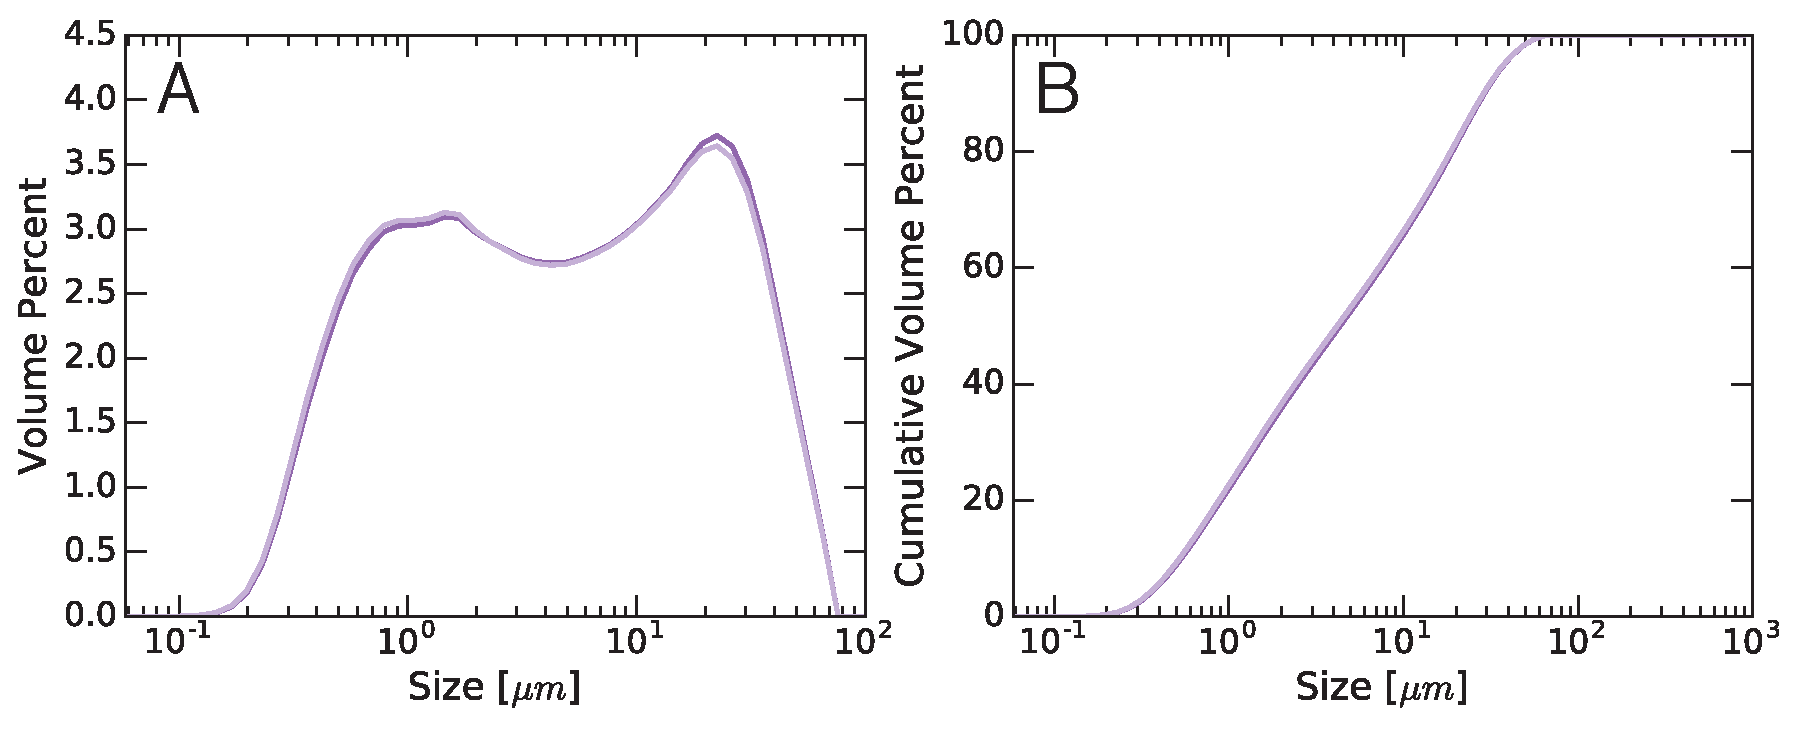
\includegraphics[scale=0.5]{chap_slow_slip_details/Figure_S1.pdf}
   	\caption{Particle size distribution (A) and cumulative size distribution (B) for Min-U-Sil 40.}
  	\label{Figure_S1}
\end{figure}
% End Figure %

\clearpage

% Figure %
\begin{figure}[H]
	\centering
		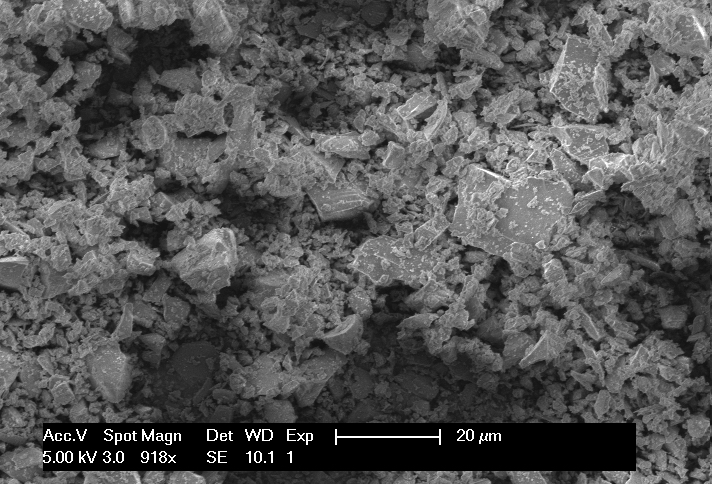
\includegraphics[scale=0.5]{chap_slow_slip_details/Figure_S2.jpg}
   	\caption{An SEM micrograph of Min-U-Sil shows its angular nature.}
  	\label{Figure_S2}
\end{figure}
% End Figure %

\clearpage

% Figure %
\begin{figure}[H]
	\centering
		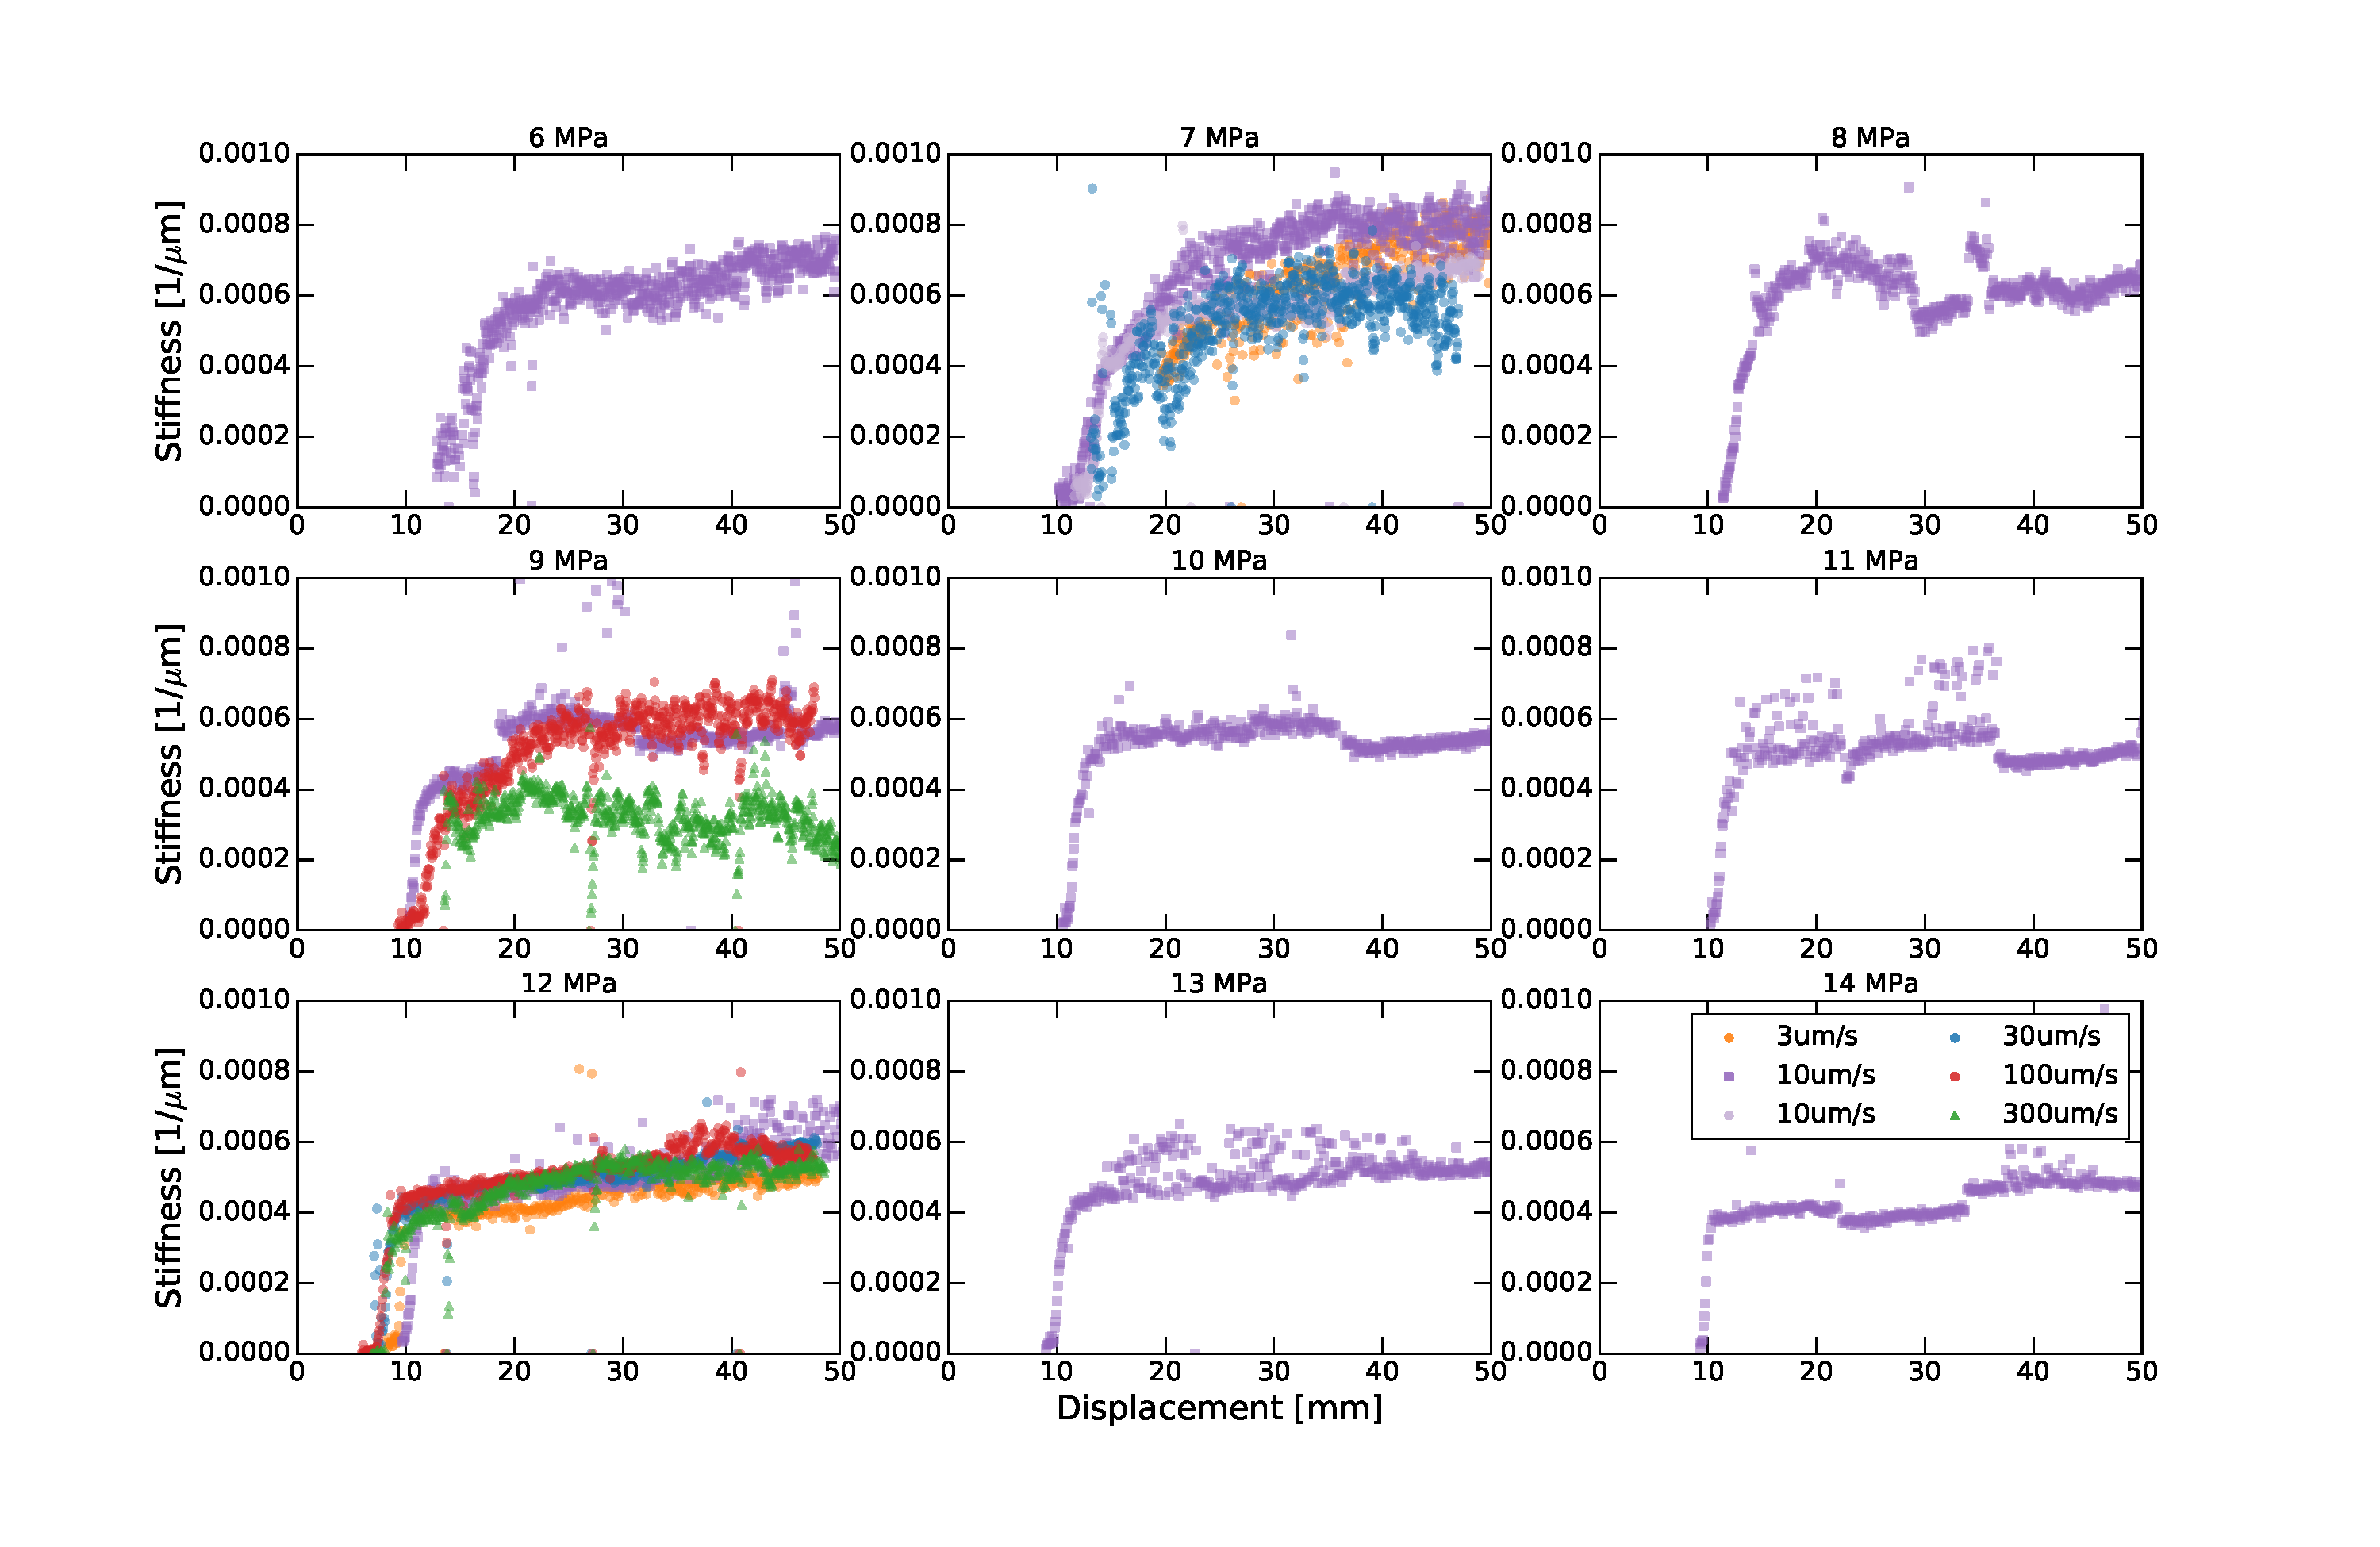
\includegraphics[scale=0.35]{chap_slow_slip_details/Figure_S3.pdf}
   	\caption{The effective stiffness of each stick-slip event at a given normal stress as a function of displacement. Notice the quick rise once events begin and asymptotic approach of a final steady-state value.}
  	\label{Figure_S3}
\end{figure}
% End Figure %

\clearpage

% Figure %
\begin{figure}[H]
	\centering
		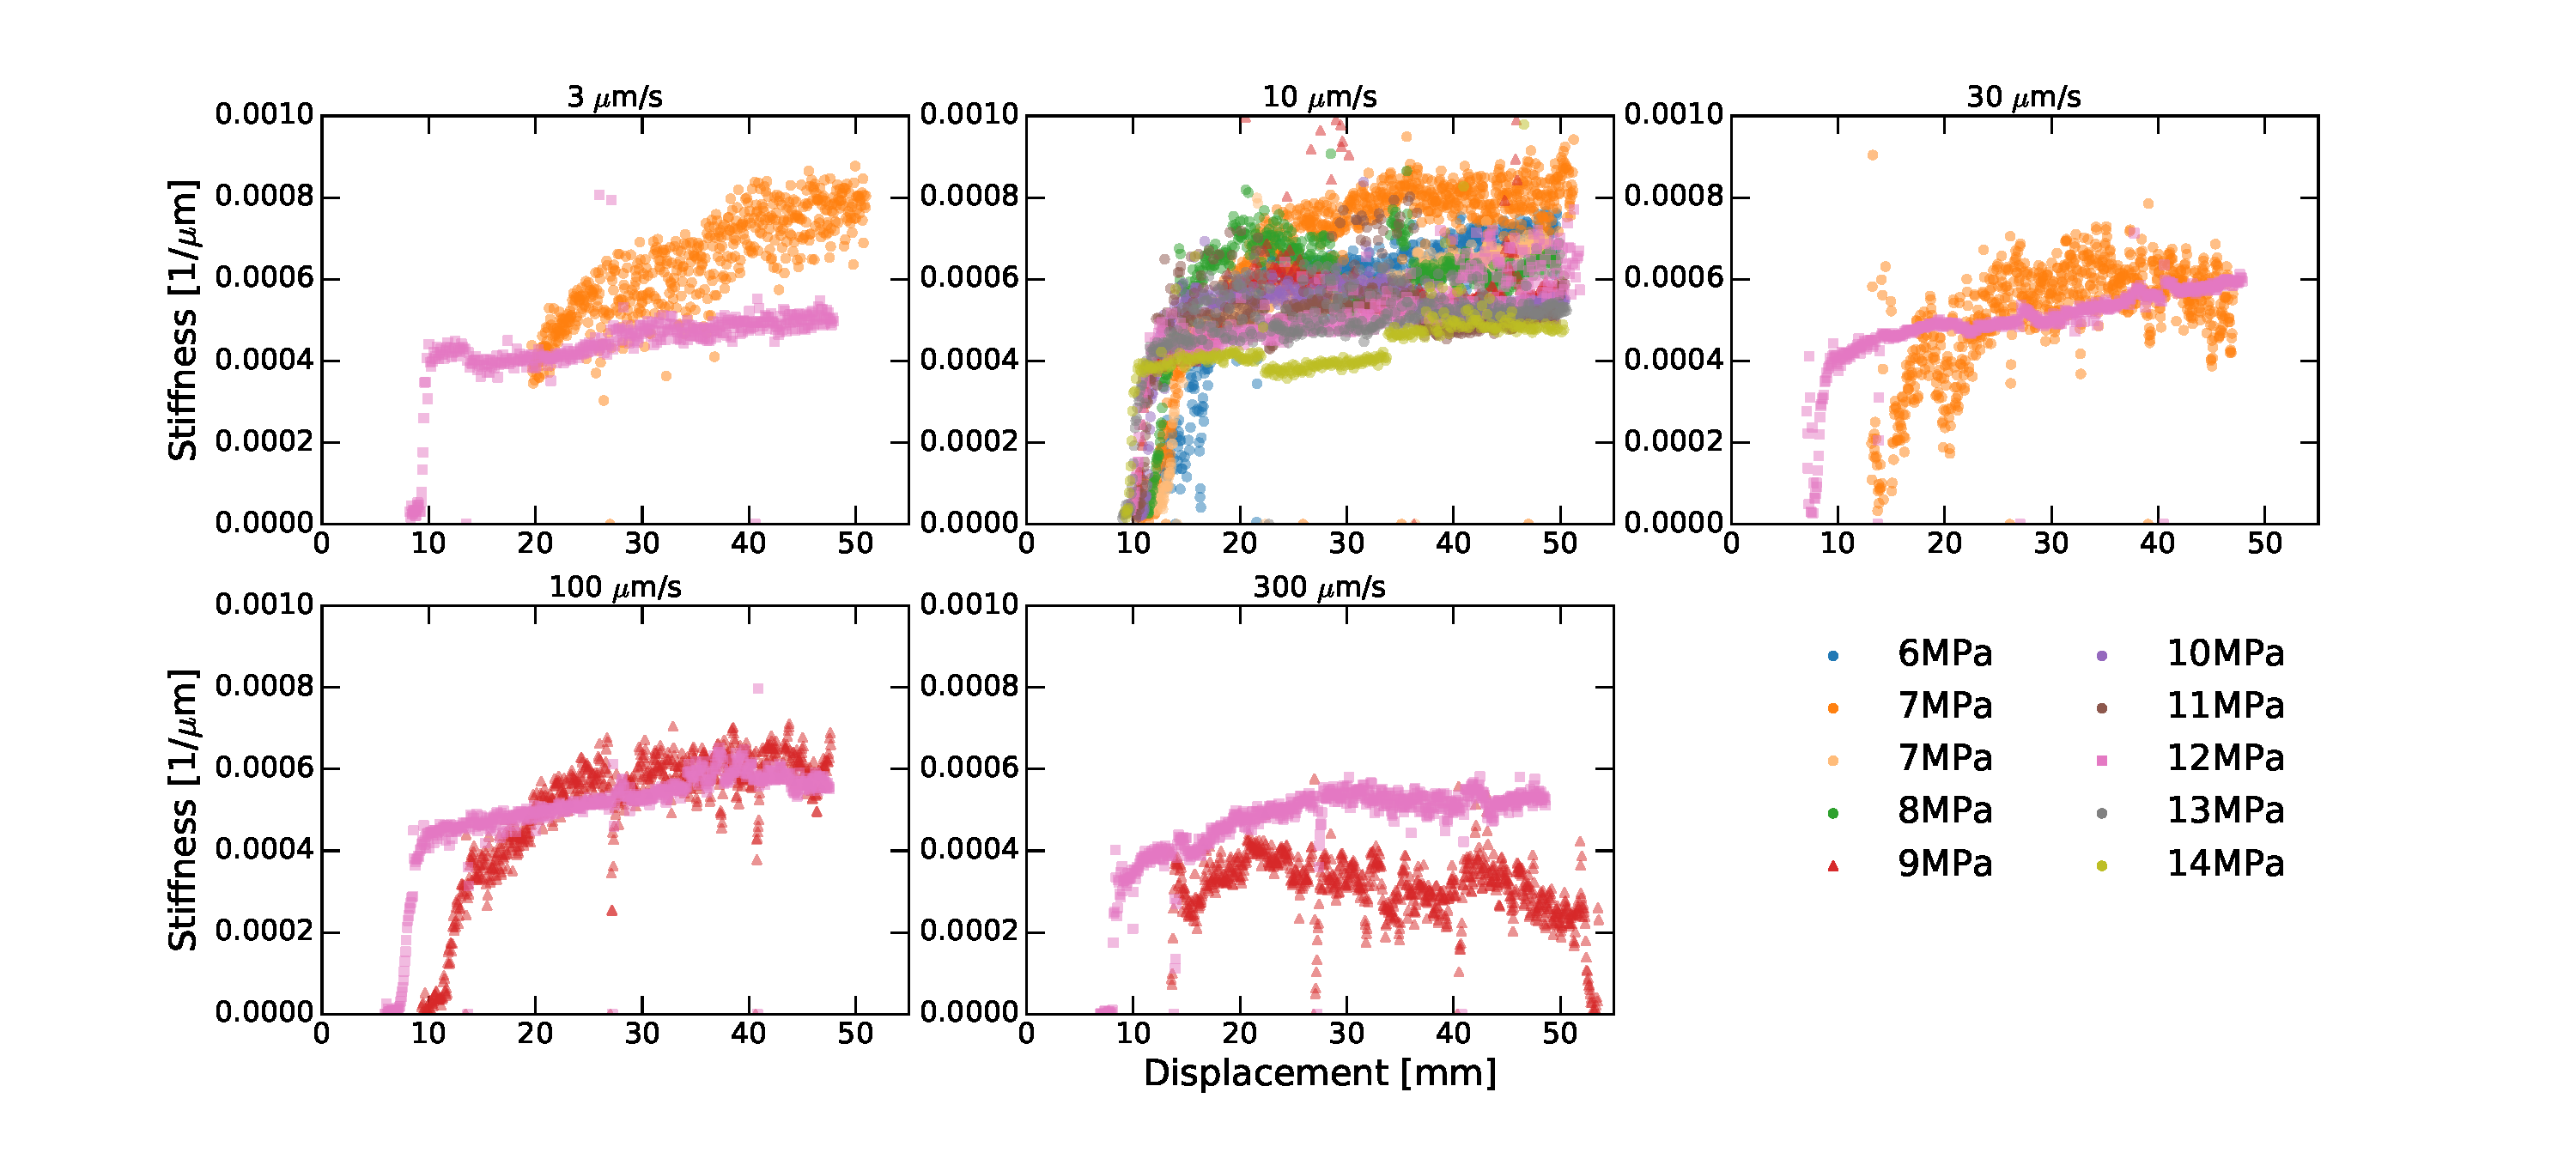
\includegraphics[scale=0.35]{chap_slow_slip_details/Figure_S4.pdf}
   	\caption{Effective stiffness of each stick-slip event at a given driving velocity as a function of displacement.}
  	\label{Figure_S4}
\end{figure}
% End Figure %

\clearpage

% Figure %
\begin{figure}
	\centering
		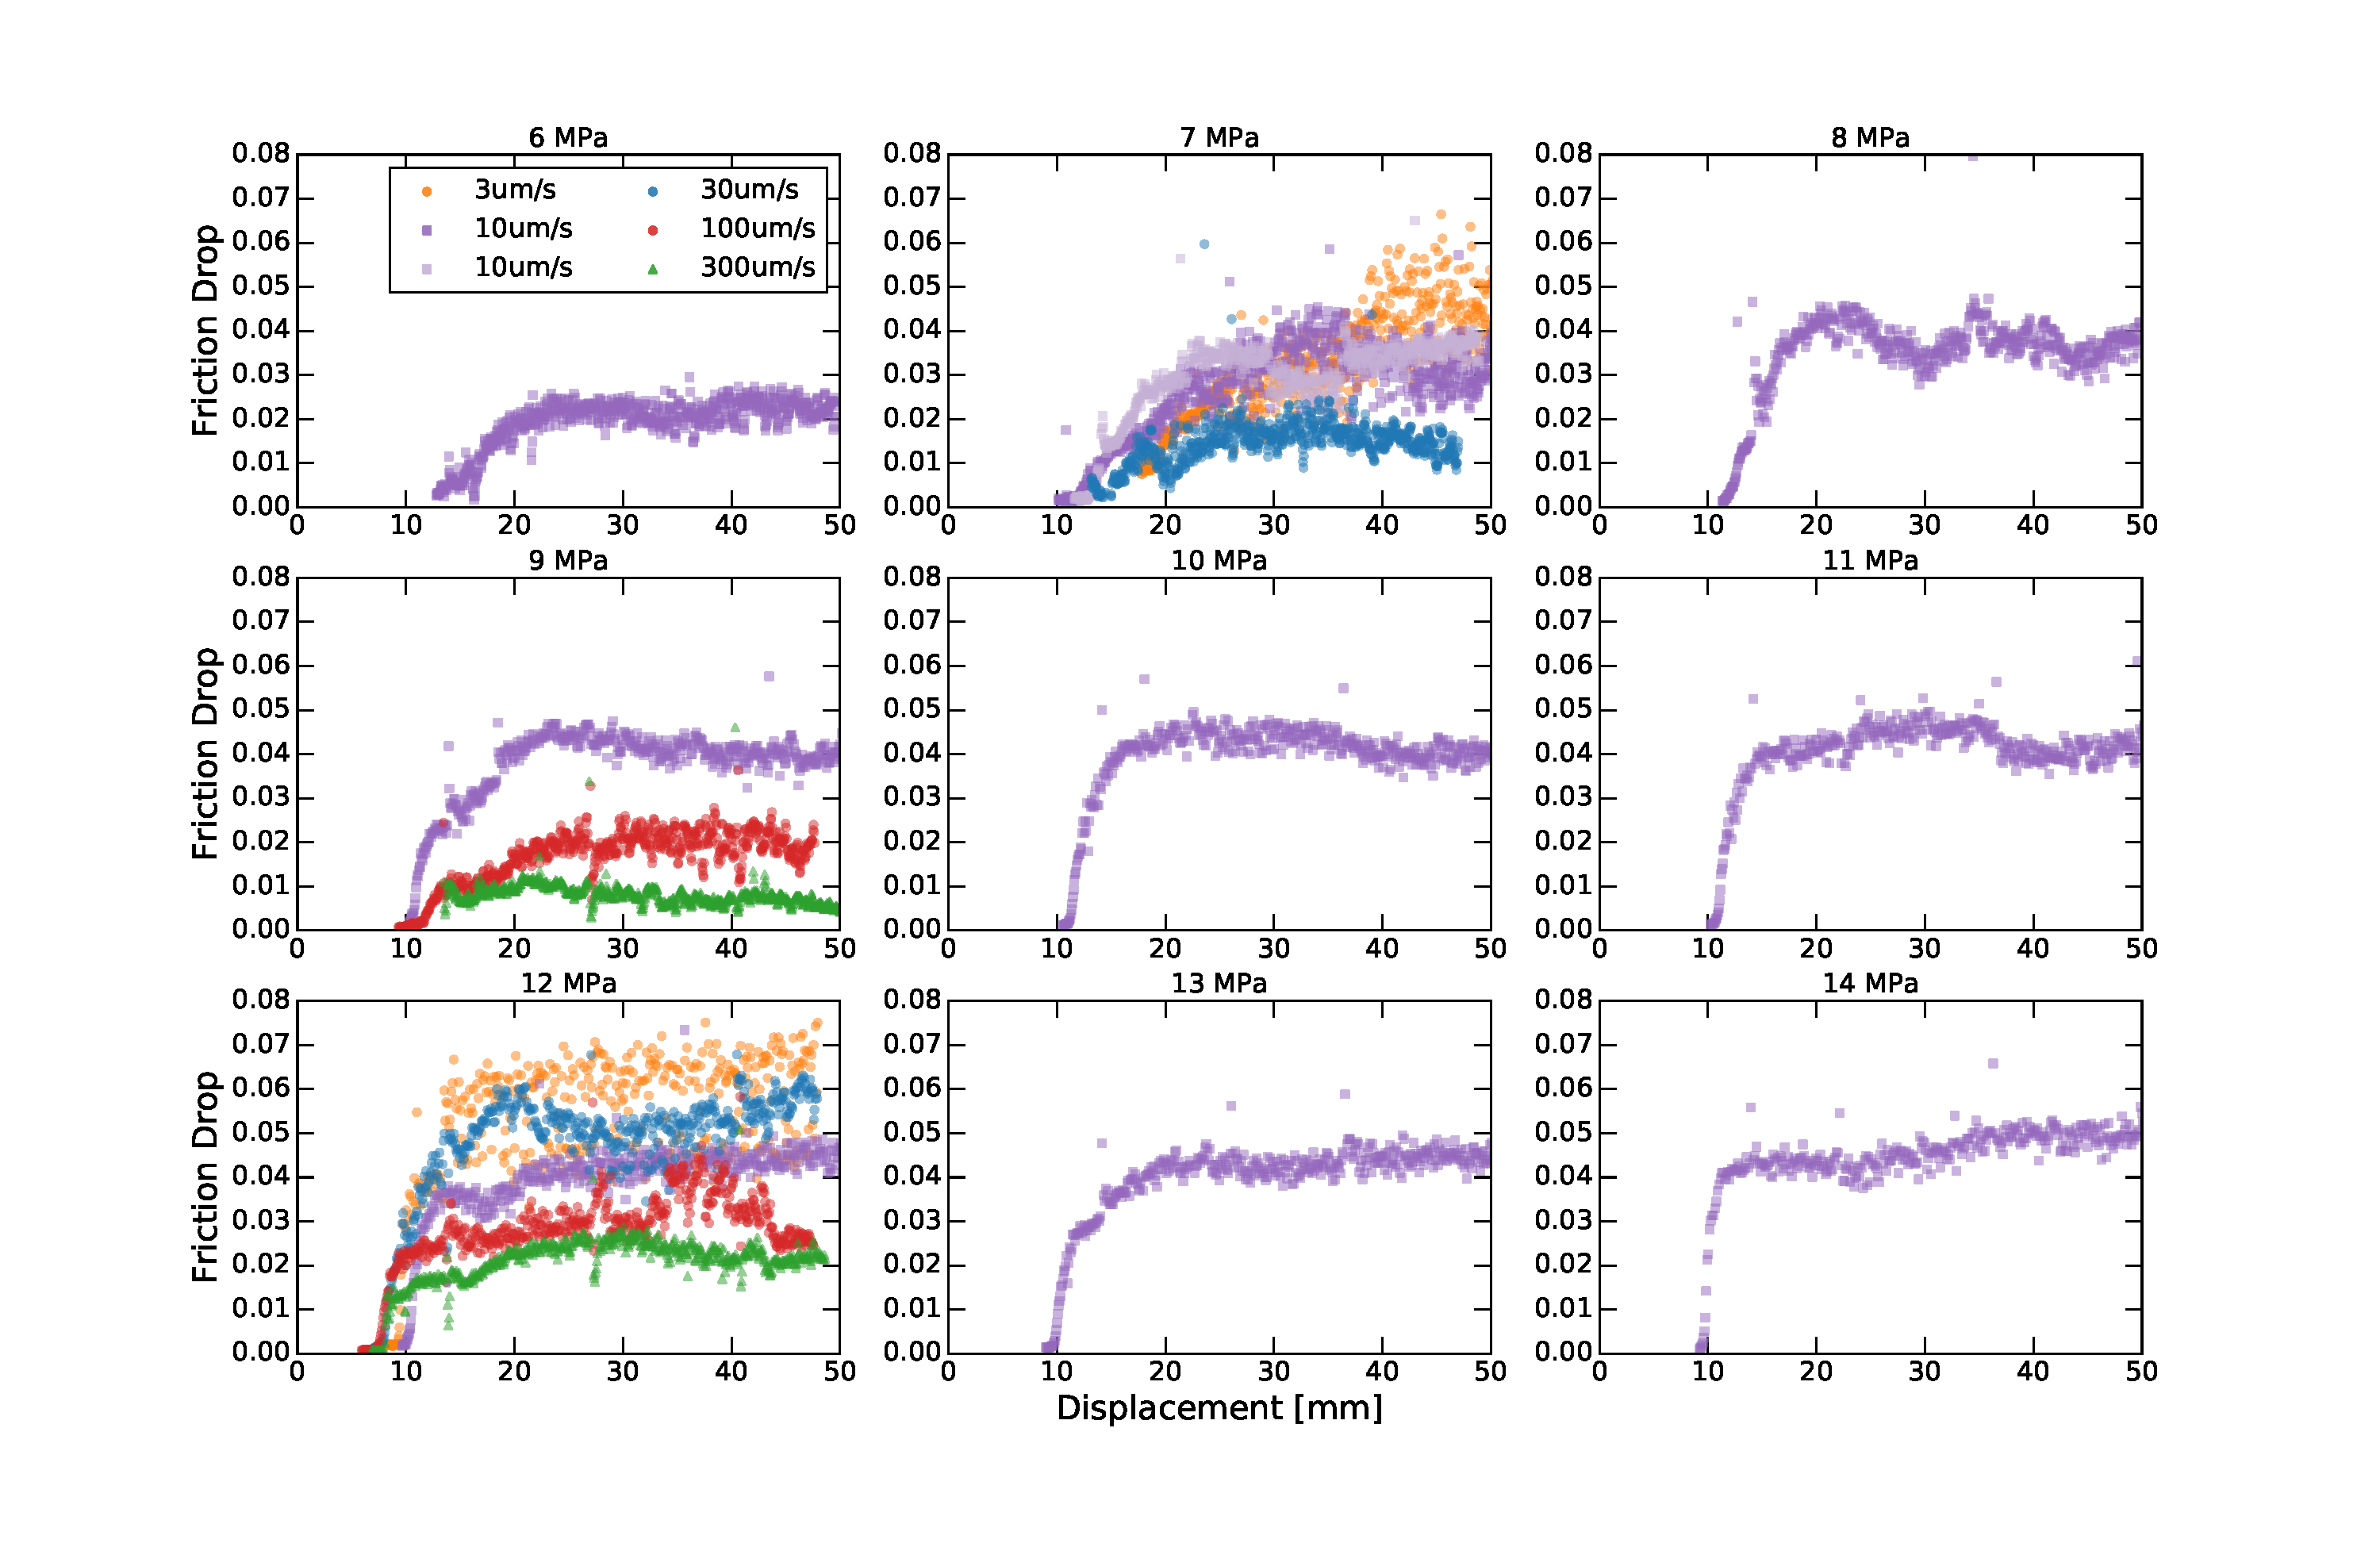
\includegraphics[scale=0.35]{chap_slow_slip_details/Figure_S5.pdf}
   	\caption{Friction drop for each stick-slip event at a given normal stress as a function of displacement.}
  	\label{Figure_S5}
\end{figure}
% End Figure %

\clearpage

% Figure %
\begin{figure}
	\centering
		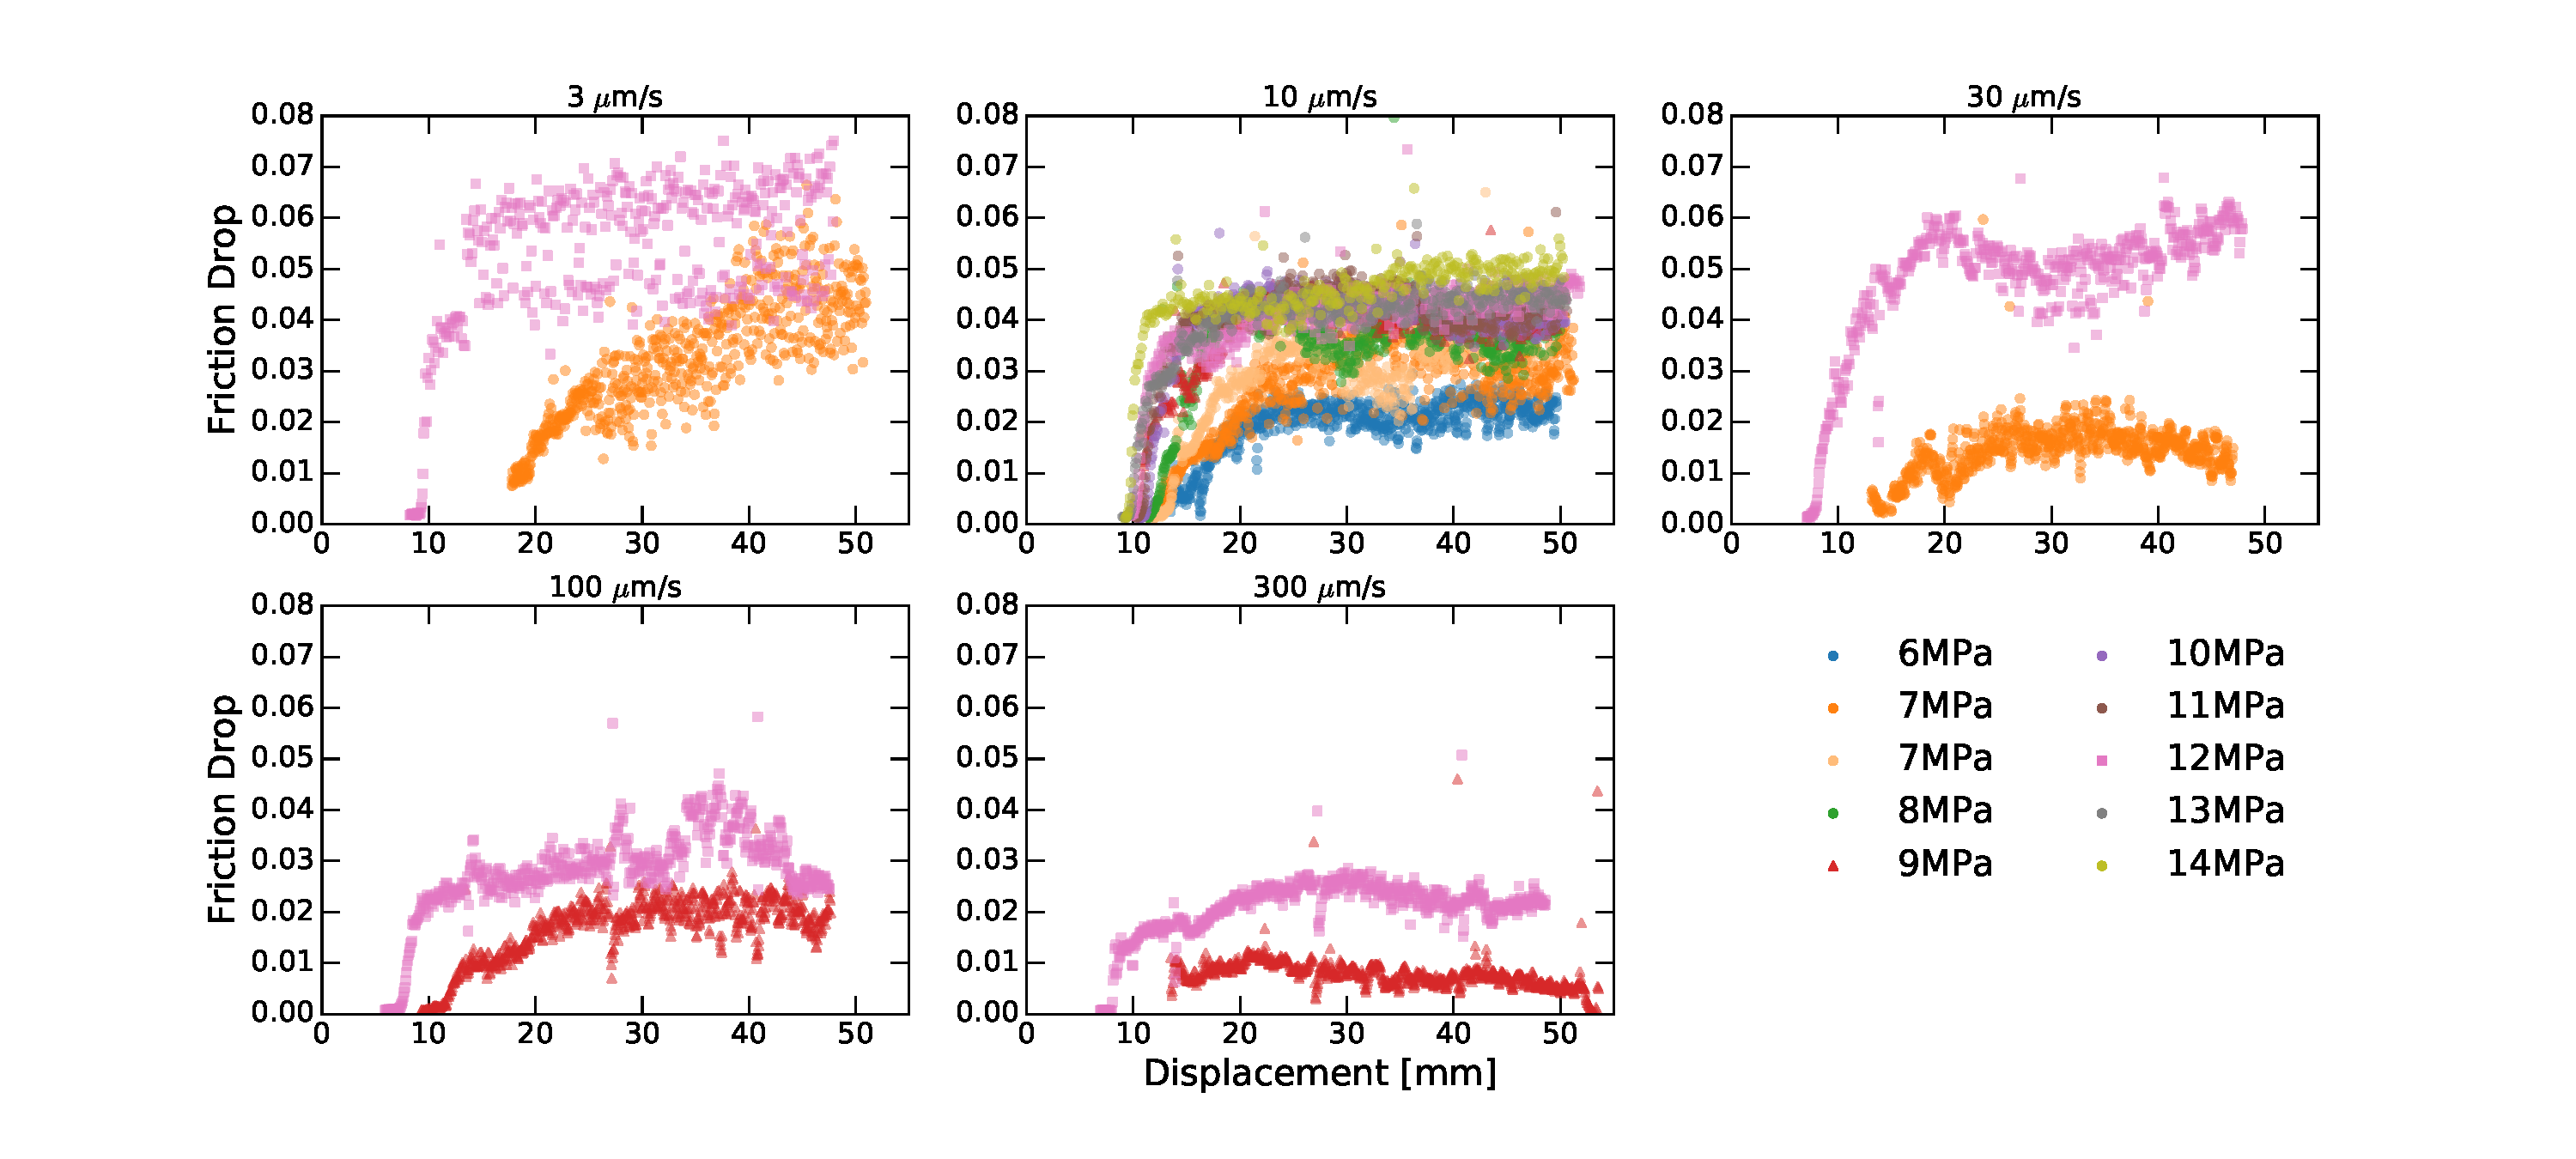
\includegraphics[scale=0.35]{chap_slow_slip_details/Figure_S6.pdf}
   	\caption{Friction drop for each stick-slip event at a given driving velocity as a function of displacement.}
  	\label{Figure_S6}
\end{figure}
% End Figure %

\clearpage

% Figure %
\begin{figure}
	\centering
		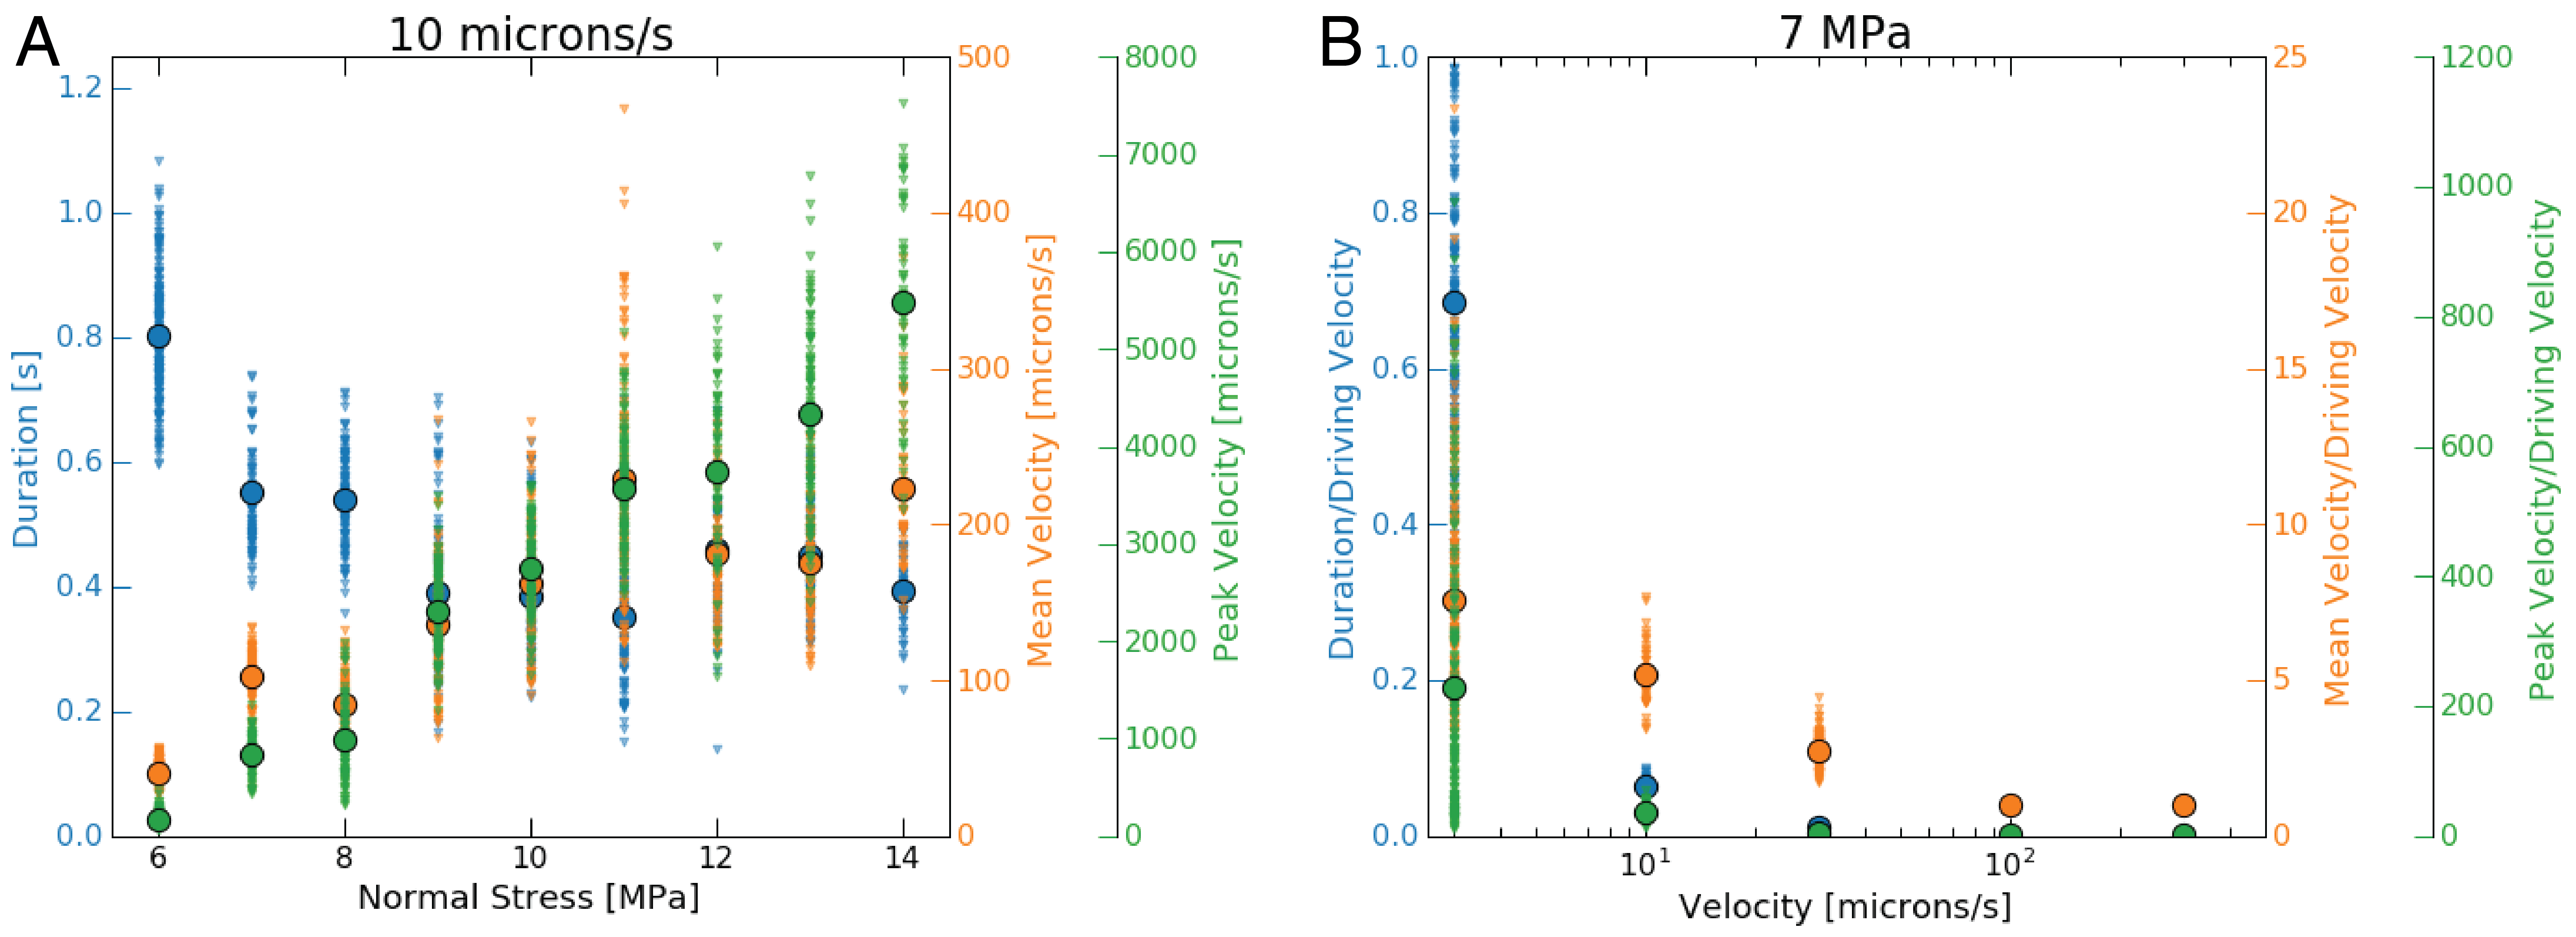
\includegraphics[scale=0.3]{chap_slow_slip_details/Figure_S7.pdf}
   	\caption{Duration, mean velocity (slip distance/slip duration), and peak velocity for events at a constant driving velocity (A) and constant normal stress (B).}
  	\label{Figure_S7}
\end{figure}
% End Figure %
